\documentclass{article}
\usepackage{arxiv}

\usepackage[utf8]{inputenc} % allow utf-8 input
\usepackage[T1]{fontenc}% use 8-bit T1 fonts
\usepackage{hyperref}   % hyperlinks
\usepackage{url}% simple URL typesetting
\usepackage{booktabs}   % professional-quality tables
\usepackage{amsfonts}   % blackboard math symbols
\usepackage{nicefrac}   % compact symbols for 1/2, etc.
\usepackage{microtype}  % microtypography
\usepackage{lipsum}
\usepackage[linesnumbered,boxed,ruled,commentsnumbered]{algorithm2e}
\usepackage{algorithmic}
\usepackage{amsmath}
\usepackage{amssymb}
\usepackage{amsthm}
\usepackage{amstext}
\usepackage{subfigure}
\usepackage{graphicx}
\usepackage{multirow}
\usepackage{listings}
\usepackage{xcolor}

\lstset{
  language = python, numbers=left, 
  numberstyle=\tiny,keywordstyle=\color{blue!70},
  commentstyle=\color{red!50!green!50!blue!50},frame=shadowbox,
  rulesepcolor=\color{red!20!green!20!blue!20},basicstyle=\ttfamily
}
\title{Large-scale Optimal Transport}


\author{
  Yifan Zhang\\
  Yuanpei College\\
  Peking University\\
}

\begin{document}
\maketitle

% keywords can be removed
\keywords{Convex Optimization \and Optimal Transport}

\tableofcontents

\section*{}

\vspace{5ex}



%%%   Section 1: Introduction   %%%
% Section 1: Introduction

\section{Introduction}

Optimal transport is widely used in the field of computer science, especially in areas as computer graphics, computer vision, medical image processing and deep learning. As the product of the intersection of multiple disciplines, it contains problems from probability, analysis, and optimization. The main objective of the research is to establish a geometric tool for efficient comparison of probability distributions, that is, the modeling of probability distributions by geometric methods and the measurement of the distance between probability distributions is a bridge connecting geometry and probability.

Take the problem given by the French mathematician Monge more than 200 years ago as an example: When two sand plates are given (each sand plate can represent a probability distribution), a sand plate can be transmitted in many ways (Transport or Reshape) to another sandbox. Based on the local cost of transmitting a single sand particle, each transport method corresponds to a global cost. The purpose of optimal transport is to find the transport solution with the lowest overall cost, so as to further establish the geometric toolset for probability distribution.

The optimal transport problem has a long and rich research history, which can be traced back to the eighteenth-century Monge mentioned above. The Russian mathematician Kantorovich gave a more practical form of relaxation in the 1940s and was further promoted in the 1990s because of a series of important mathematical theoretical achievements, including important work of French mathematician Brenier. It is particularly important that many Fields Prize winners have made important contributions in the study of optimal transport theory, such as the French mathematician Cédric Villani (The Fields Award 2010), Italian Mathematics Alessio Figalli (The Fields Award 2018), and has many important monographs \cite{book1, book2, book3, book4}. In terms of application, optimal transport has been widely used in the field of computer science, especially in computer graphics, computer vision, medical image processing, and deep learning.

In order to introduce the optimal transmission problem more concisely, we only consider the optimal transmission problem for discrete probability vectors (histograms). First, a probability vector or histogram refers to a vector $a \in \Sigma_m$ belongs to a set of probability simplex, that is,

\begin{equation}
  \Sigma_{m}:=\left\{\mathbf{a} \in \mathbb{R}_{+}^{m}: \sum_{i=1}^{m} \mathbf{a}_{i}=1\right\}
\end{equation}

Due to the computational difficulty of the optimal transport problem proposed by Monge and the limitation of this model, the Kantorovich relaxed optimal transport model has drawn attention in academia. By removing the limitation of fully deterministic transport (the quantity of the same point cannot be decomposed), Kantorovich gives a concise and effective optimal transport model. Transport is achieved through the Couplings matrix $P_+^{n \times m}$, where the set of coupling matrices is defined as

\begin{equation}
  \mathbf{U}(\mathbf{a}, \mathbf{b}) \stackrel{\text { def. }}{=}\left\{\mathbf{P} \in \mathbb{R}_{+}^{m \times n}: \mathbf{P} \mathbf{1}_{n}=\mathbf{a} \quad \text { and } \quad \mathbf{P}^{\mathrm{T}} \mathbf{1}_{m}=\mathbf{b}\right\}
\end{equation}

$\mathbf{a} \in \Sigma_m$ and $\mathbf{b} \in \Sigma_n$ are both probability vectors or histograms. The coupling matrix set is bounded and consists of $m + n$ equality constraints, which can be regarded as a convex polyhedron. 

Kantorovich optimal transmission problem can be defined as

\begin{equation}
  \mathcal{L}_{\mathbf{C}}(\mathbf{a}, \mathbf{b}):=\min _{\mathbf{P} \in \mathbf{U}(\mathbf{a}, \mathbf{b})}\langle\mathbf{C}, \mathbf{P}\rangle:=\sum_{i, j} \mathbf{C}_{i j} \mathbf{P}_{i j}
\end{equation}

Where $C \in \mathbb{R}^{n \times m}$ represents the cost matrix and $C_{ij}$ represents the cost required to transfer from $i$ to $j$. The Kantorovich optimal transport problem is a linear programming problem, and the problem does not necessarily have a unique solution. The importance of the optimal transport problem is not only in itself, it provides a way to meaningfully characterize the distance between probability vectors or histograms.

\vspace{5ex}
\begin{figure}[htbp]
  \centering
  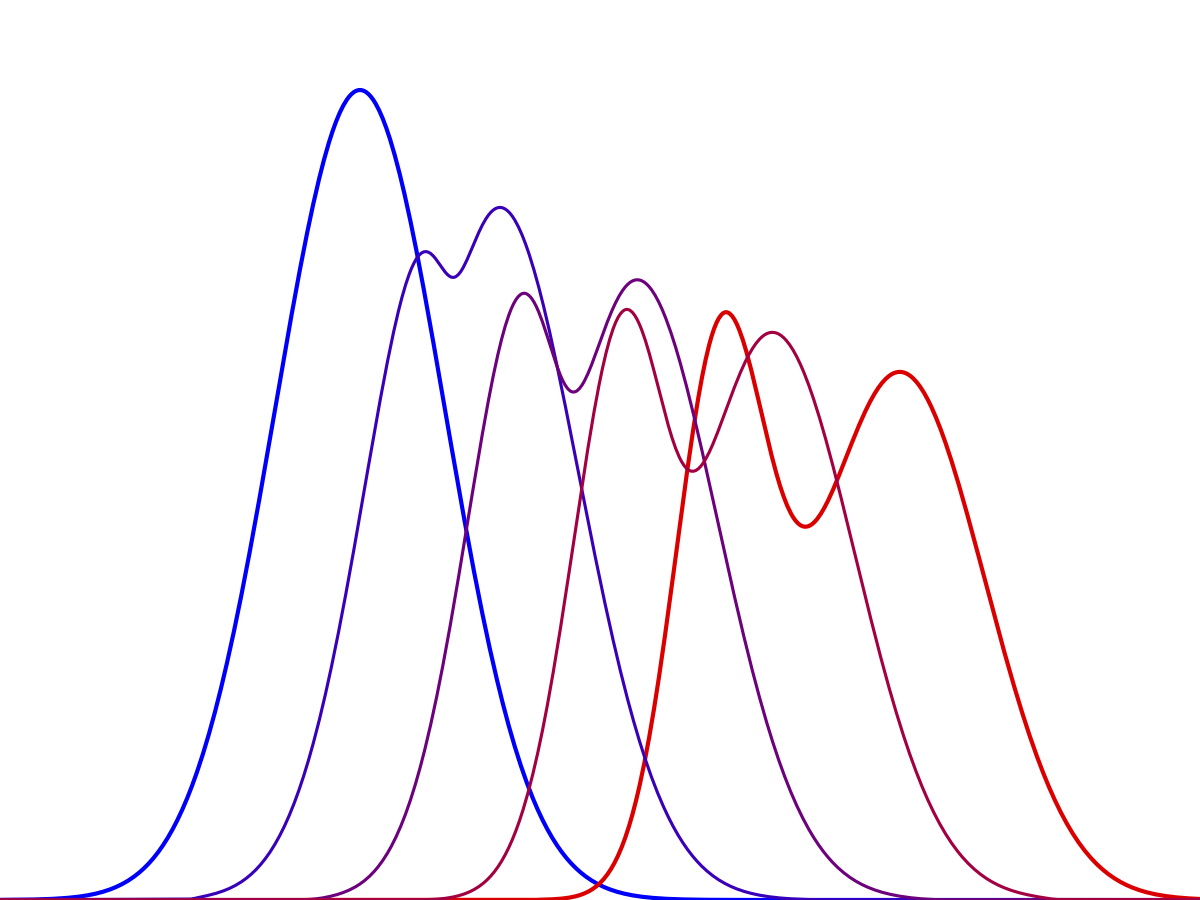
\includegraphics[width=0.8\linewidth]{img/ot}
  \label{fig:ot}
  \caption{Illustration of Optimal Transport Interpolation}
\end{figure}


%%%   Section 2: Standard Form LP   %%%
% Section 2: standard form LP

\clearpage
\section{Standard Form LP}
\begin{equation}
    \begin{aligned}
      \min _{\pi \in \mathbb{R}^{m \times n}} & \sum_{i=1}^{m} \sum_{j=1}^{n} c_{i j} \pi_{i j} \\
      \text { s.t. } & \sum_{j=1}^{n} \pi_{i j}=\mu_{i}, \quad \forall i=1, \ldots, m \\
      & \sum_{i=1}^{m} \pi_{i j}=\nu_{i}, \quad \forall j=1, \ldots, n \\
      & \pi_{i j} \geq 0
    \end{aligned}
  \end{equation}
  
  \vspace{5ex}

\subsection{Calling Mosek and Gurobi}

The standard form can be vectorized as:
\begin{equation}
    \begin{aligned}
      \min _{\pi \in \mathbb{R}^{m \times n}} & c^T \pi \\
      \text { s.t. } & A \pi = b \\
      & \pi_{i j} \geq 0
    \end{aligned}
  \end{equation}

where 
$$
c=\left(c_{11}, c_{21}, \dots c_{n 1}, \dots, c_{1 n}, \dots c_{n n}\right)^{T}
$$

$$
\pi=\left(\pi_{11}, \pi_{21}, \ldots \pi_{n 1}, \ldots, \pi_{1 n}, \ldots \pi_{n n}\right)^{T}
$$

$$
A=\left(\begin{array}{ccc}
    {I_{m}} & {\cdots} & {I_{m}} \\
    {E_{1}} & {\cdots} & {E_{n}}
    \end{array}\right),\left(E_{j}\right)_{s t}=\delta_{s j}
$$

$$
b=\left(\mu_{1}, \dots \mu_{m}, \nu_{1}, \dots \nu_{n}\right)^{T}
$$

Then we could directly call linear programming solvers provided by Mosek and Gurobi.

\subsection{First Order Method: ADMM}
For convenience, we reformulate the original primal problem as:

\begin{equation}  
\begin{array}{rl}
{\mathrm{(primal)}} & {\min_\pi \sum_{i=1}^{m} \sum_{j=1}^{n} c_{i j} \pi_{i j} + I_{\mathbb{R}_+^{m\times n}}(\pi^\dagger)} \\
{\text { subject to }} & {\sum_{j=1}^{n} \pi_{i j}=\mu_{i} \forall i=1, \ldots, m} \\
{} & {\sum_{i=1}^{m} \pi_{i j}=\nu_{j} \forall j=1, \ldots, n} \\
& \pi = \pi^{\dagger}
\end{array}
\end{equation}

Then we have the augmented Lagrangian: 

\begin{equation}
  \begin{aligned}L(\pi, \pi^{\dagger}, u, v, w)=& \min_\pi \sum_{i=1}^{m} \sum_{j=1}^{n} c_{i j} \pi_{i j} + I_{\mathbb{R}_+^{m\times n}}(\pi^\dagger) \\&+\sum_{i=1}^{m} u_{i}\left(\mu_{i}-\sum_{j=1}^{n} \pi_{i j}\right)+\sum_{j=1}^{n} v_{j}\left(\nu_{j}-\sum_{i=1}^{m} \pi_{i j}\right)+\sum_{i=1}^{m} \sum_{j=1}^{n} w_{i j}\left(\pi_{i j}-\pi^{\dagger}_{i j}\right) \\&+\frac{\rho}{2} \sum_{i=1}^{m}\left(\mu_{i}-\sum_{j=1}^{n} \pi_{i j}\right)^{2}+\frac{\rho}{2} \sum_{j=1}^{n}\left(\nu_{j}-\sum_{i=1}^{m} \pi_{i j}\right)^{2}+\frac{\rho}{2} \sum_{i=1}^{m} \sum_{j=1}^{n}\left(\pi_{i j}-\pi^{\dagger}_{i j}\right)^{2}\end{aligned}
\end{equation}

$\partial_{\pi_{ij}} L = 0 $ gives: 

\begin{equation}
  \sum_{k=1}^{n} \pi_{i k}+\sum_{k=1}^{m} \pi_{k j}+\pi_{i j}=\frac{1}{\rho}\left(-e_{i j}+u_{i}+v_{j}-c_{i j}\right)+\mu_{i}+\nu_{j}+\pi_{ij}^{\dagger}
\end{equation}

$\partial_{\pi^{\dagger}_{ij}} = 0$ gives:

\begin{equation}
  {\pi^{\dagger}_{ij}} = (\pi_{ij} + \frac{w_{ij}}{\rho})_+
\end{equation}

\vspace{2ex}
    \begin{algorithm}[htbp]
        \SetAlgoNoLine
        \caption{ADMM method for primal problem} 
        \KwIn{parameters $\mu$, $\nu$, $c$}
        \KwIn{step size $\alpha$, penalty $\rho$}
        Initialize variables $\pi, \pi^{\dagger} = \boldsymbol{0}$\\
        Initialize variables $u, v, w = \boldsymbol{0}$\\
        \While{ stopping criterion not met } 
        {  
            Update $\pi$: $\boldsymbol{\pi} \leftarrow \operatorname{argmin}_{\pi} L(\pi, \pi^{\dagger}, u, v, w)$\\
            Update $\pi^{\dagger}$: $\boldsymbol{\pi}^{\dagger} \leftarrow \operatorname{argmin}_{\pi^{\dagger}} L(\pi, \pi^{\dagger}, u, v, w)$\\
            Update $u$: $\boldsymbol{u} \leftarrow u + \rho\cdot \alpha (\mu - \sum_j \pi_{ij})$\\
            Update $v$: $\boldsymbol{v} \leftarrow v + \rho\cdot \alpha (\nu - \sum_i \pi_{ij})$\\
            Update $w$: $\boldsymbol{w} \leftarrow w + \rho\cdot \alpha (\pi - \pi^{\dagger})$\\
        }
    \end{algorithm}


%%%   Section 3: Problem Background  %%%
% Section 3: Problem Background

\section{Problem Background}

For the present context it is sufficient to restrict ourselves to optimal transport on $\mathbb {R}^d$. Let $X$,  $Y$ be subsets of $\mathbb{R}^d$ and let $\mu$ and $\nu$ be probability measures on $X$ and $Y$, respectively. In this paper we will always have X = Y , but using different notation for domain and target space makes definitions easier to grasp.

Transport map $T$ is any (measurable) map $X  \rightarrow Y$ that transforms the measure $\mu$ into the measure $\nu$. More precisely it satisfies $\mu(T^{-1}(B)) = \nu(B)$ for every measurable $B \subset Y$ . A transference plan is a measure $\pi$ on $X \times Y$ with marginals $\pi(\cdot \times Y) = \mu$ and $\pi(X \times \cdot) = \nu$. The set of transference plans from $\mu$ to $\nu$ is denoted by $\Pi(\mu, \nu)$. Any transport map $T$ from $\mu$ to $\nu$ defines a transference plan $\pi_T$ from $\mu$ to $\nu$ as the unique measure satisfying $\pi_{T}(A \times B)=\mu\left(A \cap T^{-1}(B)\right)$ for all measurable $A \subset X$ and $B \subset Y$. Not every transference plan $\pi$ can be represented in this way, because transference plans allow mass from one site $x \in X$ to be split between multiple destinations, which is not possible under a transport map. Figure 1 shows such an example.

\begin{figure}[htbp]
  \centering
  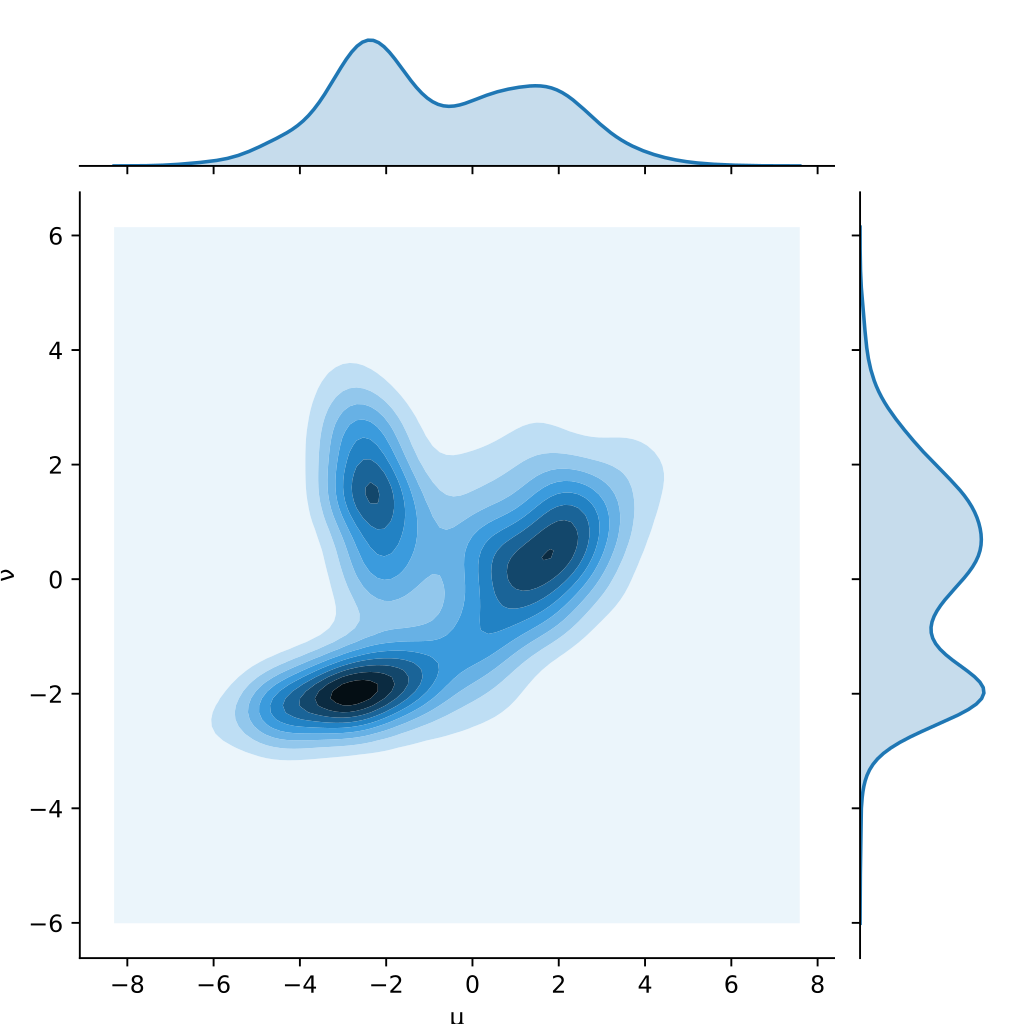
\includegraphics[width=0.8\linewidth]{img/1d_ot}
  \label{fig:ot}
  \caption{Two one-dimensional distributions $\mu$  and $\nu$ , plotted on the x and y axes, and one possible joint distribution that defines a transport plan between them.}
\end{figure}

We assume that the cost of transporting a unit mass from $x \in X$ to $y \in Y$ is $c_p(x,y) = \|x-y\|^p$ for some $p \geq 1$. The minimum cost for transferring $\mu$ to $\nu$ is then given by 

\begin{equation}
  C_p (\mu, \nu) = \min_{x \in \Pi(\mu,\nu)} \|x-y\|^p d\pi(x,y)
\end{equation}

Taking the $p^{th}$ root, we obtain the Wasserstein metric $W_p$. More precisely we have 

\begin{equation}
  W_p(\mu, \nu) = C_p(\mu, \nu)^{1/p}
\end{equation}

for and measures $\mu$ and $\nu$ that satisfy $\int_{X}\|x\|^{p} d \mu(x)<\infty$ adn $\int_{Y}\|y\|^{p} d \nu(y)<\infty$. In order to evaluate the Wasserstein metric, we need to find an optimal solution to $C_p(\mu,\nu)$, i.e., a minimizing transference plan $\pi$. This problem is often referred to as the Kantorovich formulation of optimal transport. Note that by Theorem 4.1 in [29] a minimizing always exists. However, it neither has to be unique nor representable in terms of an optimal transport map.

Often one would like to compare data sets that are available as images from a certain source, e.g. real photography, astronomical imagery, or microscopy data. We may think of such images as discrete measures on a grid. For example, tiny clippings from STED microscopy images of mitochondrial networks. A question of interest might be whether both images stem from the same part of the network, which can in principle be answered by finding an optimal transference plan (third panel in Figure 1) and computing the Wasserstein distance. Note that this coarse resolution is not representative for a serious analysis, but was only chosen for illustrative purposes.

Assume now that we have discrete measures of the form $\mu = \sum_{i=1}^m \mu_i \delta_{x_i}$ and $\nu = \sum_{j = 1}^n \nu_i \delta_{y_j}$ and write $c_{ij} = ||x_i - y_j||^p$. In what follows, we always have $m = n$, and $(x_i)_{1 \leq i \leq m} = (y_j)_{i\leq j \leq n}$ form a regular square grid in $R^2$, but since it is more intuitive, we keep different notation for source locations and target locations. Let $\pi_{ij}$ be the amount of mass transported from $x_i$ to $y_j$. Then, the problem can be rewritten as a linear program: 

\begin{equation}
  \begin{array}{rl}{\mathrm{(primal)}} & {\min_\pi \sum_{i=1}^{m} \sum_{j=1}^{n} c_{i j} \pi_{i j}} \\{\text { subject to }} & {\sum_{j=1}^{n} \pi_{i j}=\mu_{i},\quad \forall i=1, \ldots, m} \\{} & {\sum_{i=1}^{m} \pi_{i j}=\nu_{j},\quad \forall j=1, \ldots, n} \\{} & {\pi_{i j} \geq 0}\end{array}
\end{equation}

Note that this primal form has $mn$ variables which leads to computational difficulties, we can deduct the dual form of this problem as:

\begin{equation}
  \begin{array}{rl}{\mathrm{(dual)}} & {\max _{u, v} \sum_{i=1}^{m} \mu_{i} u_{i}+\sum_{j=1}^{n} \nu_{j} v_{j}} \\{\text { subject to }} & {c_{ij} - u_i - v_j \geq 0\qquad\forall i=1, \ldots, m \quad j = 1,\cdots,n}\end{array}
\end{equation}

Though only $m + n$ variables left, there still exist $mn$ constraints.


%%%   Section 4: Algorithms  %%%
% Section 4: Algorithms
\section{Algorithms}




\subsection{ADMM method for dual problem}
For convenience, introducing relaxation variables, we reformulate the dual problem as:

\begin{equation}
  \begin{array}{rl}
    {\mathrm{(dual)}} & {\min -_{u,v} \sum_{i=1}^{m} \mu_{i} u_{i}-\sum_{j=1}^{n} \nu_{j} v_{j}} + I_{\mathbb{R}_+^{m\times n}}(\xi)\\
    {\text { subject to }} & {c_{ij} - u_i - v_j -\xi_{ij}= 0\qquad\forall i=1, \ldots, m \quad j = 1,\cdots,n}
    \end{array}
\end{equation}

Then we have the augmented Lagrangian:

\begin{equation}
  \begin{aligned}L(u, v, \xi, w)=&-\sum_{i=1}^{m} \mu_{i} u_{i}-\sum_{j=1}^{n} \nu_{j} v_{j} + I_{\mathbb{R}_+^{m\times n}}(\xi)\\&+\sum_{i=1}^{m} \sum_{j=1}^{n} w_{i j}\left(c_{i j}-u_{i}-v_{j}-\xi_{i j}\right)+\frac{\rho}{2} \sum_{i=1}^{m} \sum_{j=1}^{n}\left(c_{i j}-u_{i}-v_{j}-\xi_{i j}\right)^{2}\end{aligned}
\end{equation}

$\partial_{\xi_{ij}} L = 0$ gives:

\begin{equation}
  \xi_{ij} = (c_{ij} - u_i - v_j + \frac{w_{ij}}{\rho})_+
\end{equation}

$\partial_{u_i}L = 0$ gives:

\begin{equation}
  u_i = \frac{1}{n}\left(\frac{\mu_{i}+\sum_{j=1}^{n} w_{i j}}{\rho}+\sum_{j=1}^{n}\left(c_{i j}-v_{j}-\xi_{i j}\right)\right)
\end{equation}

$\partial_{v_j} L = 0$ gives:
\begin{equation}
  v_j = \frac{1}{n}\left(\frac{\nu_{j}+\sum_{i=1}^{m} w_{i j}}{\rho}+\sum_{i=1}^{m}\left(c_{i j}-u_{j}-\xi_{i j}\right)\right)
\end{equation}

\vspace{2ex}
    \begin{algorithm}[htbp]
        \SetAlgoNoLine
        \caption{ADMM method for dual problem} 
        \KwIn{parameters $\mu$, $\nu$, $c$}
        \KwIn{step size $\alpha$, penalty $\rho$}
        Initialize variables $u, v = \boldsymbol{0}$\\
        Initialize variables $\xi, w = \boldsymbol{0}$\\
        \While{ stopping criterion not met } 
        {  
            Update $u$: $\boldsymbol{u} \leftarrow \operatorname{argmin}_{u} L(u, v, \xi, w)$\\
            Update $\pi^{\dagger}$: $\boldsymbol{\pi}^{\dagger} \leftarrow \operatorname{argmin}_{u} L(u, v, \xi, w)$\\
            Update $\xi$: $\boldsymbol{\xi} \leftarrow \operatorname{argmin}_{\xi} L(u, v, \xi, w)$\\
            Update $w$: $\boldsymbol{w} \leftarrow w + \rho\cdot \alpha (\pi - \pi^{\dagger})$\\
        }
    \end{algorithm}

\subsection{Entropic Regularization Methods}
The Kullback-Leibler divergence is defined as 

\begin{equation}
  \mathbf{K L}(\mathbf{P} | \mathbf{Q}) \stackrel{\text { def. }}{=} \sum_{i, j} \mathbf{P}_{i, j} \log \left(\frac{\mathbf{P}_{i, j}}{\mathbf{Q}_{i, j}}\right)-\mathbf{P}_{i, j}+\mathbf{Q}_{i, j}
\end{equation}

with the convention $0 \log(0) = 0$ and $\mathbf{K L}(\mathbf{P} | \mathbf{Q}) = +\infty$ if there exists some $(i, j)$ such that $\mathbf{Q}_{i,j} = 0$ but $\mathbf{P}_{i,j} \neq 0$. The special case $\mathbf{K L}(\mathbf{P} | \mathbf{1})$ corresponds to minus the Shannon-Boltzmann entropy. The function $\mathbf{K L}(\cdot | \mathbf{Q})$ is strongly convex, because its hessian is $\partial^{2} \mathbf{K L}(\mathbf{P} | \mathbf{Q})=\operatorname{diag}\left(1 / \mathbf{P}_{i, j}\right)$ and $\mathbf{P}_{i,j} \leq 1$.

The idea of the entropic regularization of optimal transport is to use $\mathbf{KL}$ as a regularizing function to obtain approximate solutions to the original transport problem:

\begin{equation}
  \label{eq:entropy_regularization}
  \mathrm{L}_{\mathbf{C}}^{\varepsilon}(\mathbf{\mu}, \mathbf{\nu}) \stackrel{\text { def. }}{=} \min _{\mathbf{P} \in \mathbf{U}(\mathbf{\mu}, \mathbf{\nu})}\langle\mathbf{P}, \mathbf{C}\rangle+\varepsilon \mathbf{K L}(\mathbf{P} | \mathbf{\mu} \otimes \mathbf{\nu})
\end{equation}

Here we used as a reference measure for the relative entropy $\mathbf{\mu} \otimes \mathbf{\nu}=\left(\mathbf{\mu}_{i} \mathbf{\nu}_{j}\right)_{i, j}$. This choice of normalization, specially in this discrete setting, has no importance for the selection of the optimal $\mathbf{P}$ since it only affects the objective by a constant, indeed for $\mathbf{P} \in \mathbf{U}(\mathbf{\mu}, \mathbf{\nu})$, one has 

\begin{equation}
  \mathbf{K L}(\mathbf{P} | \mathbf{\mu} \otimes \mathbf{\nu})=\mathbf{K} \mathbf{L}\left(\mathbf{P} | \mathbf{\mu}^{\prime} \otimes \mathbf{\nu}^{\prime}\right)+\mathbf{K} \mathbf{L}\left(\mathbf{\mu}^{\prime} \otimes \mathbf{\nu}^{\prime} | \mathbf{\mu} \otimes \mathbf{\nu}\right)
\end{equation}

At this time, the approximate optimal transport problem has the $\epsilon$-strongly convex objective function, so it has a unique solution. Theoretically, As $\epsilon$ approaches 0, the optimal solution of the approximate optimal transport problem $\mathbf{P}_{\epsilon}$ converges to the optimal solution of the Kantorovich optimal transport problem. At this time, we can use the Sinkhorn algorithm to solve this problem with entropy regularization.

\begin{figure}[htbp]
  \centering
  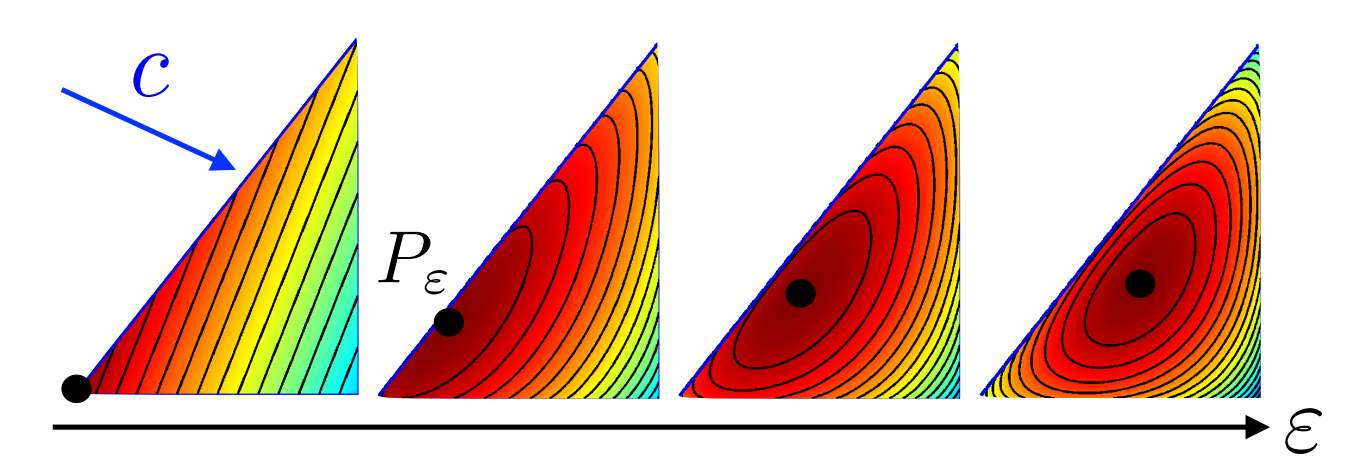
\includegraphics[width=0.9\linewidth]{img/regularized}
  \label{fig:regularized}
  \caption{Impact of $\epsilon$ on the optimization of a linear function on the simplex}
\end{figure}

\subsection{Sinkhorn Algorithm}
The following theorem [4] shows that the solution of \ref{eq:entropy_regularization} has a specific form, which can be parameterized
using $m + n$ variables. That parameterization is therefore essentially dual, in the sense that a coupling $\mathbf{P}$ in
$\mathbf{U}(a, b)$ has $nm$ variables but $n + m$ constraints.

\paragraph{Theorem}
  $\mathbf{P}$ is the unique solution to \ref{eq:entropy_regularization} if and only if there exists $(u, v) \in R$ such that
  
  \begin{equation}
    \label{eq:thm1}
    \forall(i, j) \in [m] \times [n], \quad \mathbf{P}_{i, j}=\mathbf{u}_{i} \mathbf{K}_{i, j} \mathbf{v}_{j}
  \end{equation}
  and $\mathbf{P} \in \mathcal{U}(\mathbf{\mu}, \mathbf{\nu})$.

This can be proved by introducing two dual variables $\mathbf{f} \in \mathbb{R}^{m}, \mathbf{g} \in \mathbb{R}^{n}$ for each marginal constraint, the Lagrangian of \ref{eq:entropy_regularization}
reads

\begin{equation}
  \mathcal{E}(\mathbf{P}, \mathbf{f}, \mathbf{g})=\langle\mathbf{P}, \mathbf{C}\rangle+\varepsilon \mathbf{K} \mathbf{L}(\mathbf{P} | \mathbf{\mu} \otimes \mathbf{\nu})+\left\langle\mathbf{f}, \mathbf{\mu}-\mathbf{P} \mathbf{1}_{m}\right\rangle+\left\langle\mathbf{g}, \mathbf{\nu}-\mathbf{P}^{\mathrm{T}} \mathbf{1}_{n}\right\rangle
\end{equation}

Considering first order conditions (where we ignore the positivity constraint, which can be made rigorous by
showing the associated multiplier vanishes), we have

\begin{equation}
  \label{eq:partial}
  \frac{\partial \mathcal{E}(\mathbf{P}, \mathbf{f}, \mathbf{g})}{\partial \mathbf{P}_{i, j}}=\mathbf{C}_{i, j}+\varepsilon \log \left(\frac{\mathbf{P}_{i, j}}{\mathbf{\mu}_{i} \mathbf{\nu}_{j}}\right)-\mathbf{f}_{i}-\mathbf{g}_{j}=0
\end{equation}

which results, for an optimal $\mathbf{P}$ coupling to the regularized problem, in the expression $\mathbf{P}_{i, j}=\mathbf{\mu}_{i} \mathbf{\nu}_{j} e^{\frac{\mathbf{f}_{i}+\mathbf{g}_{j}-\mathbf{C}_{i, j}}{\varepsilon}}$ 
which can be rewritten in the form provided in the proposition using non-negative vectors
\begin{equation}
  \mathbf{u} \stackrel{\text { def. }}{=}\left(\mathbf{\mu}_{i} e^{\mathbf{f}_{i} / \varepsilon}\right)_{i}, \qquad \text{and} \qquad \mathbf{v} \stackrel{\text { def. }}{=}\left(\mathbf{\nu}_{j} e^{\mathbf{g}_{j} / \varepsilon}\right)_{j}
\end{equation}

The factorization of the optimal solution exhibited in Equation \ref{eq:thm1} can be conveniently rewritten in
matrix form as $P = diag(u)K diag(v)$. $\mathbf{u}, \mathbf{v}$ must therefore satisfy the following non-linear equations which
correspond to the mass conservation constraints inherent to $\mathbf{U}(a, b)$,

\begin{equation}
\operatorname{diag}(\mathbf{u}) \mathbf{K} \operatorname{diag}(\mathbf{v}) \mathbf{1}_{n}=\mathbf{\mu}, \quad \text { and } \quad \operatorname{diag}(\mathbf{v}) \mathbf{K}^{\top} \operatorname{diag}(\mathbf{u}) \mathbf{1}_{m}=\mathbf{\nu}
\end{equation}

These two equations can be further simplified, since $\operatorname{diag}(v) \mathbf{1}_n$ is $v$, and the multiplication of $\operatorname{diag}(u)$ times $\mathbf{Kv}$ is

\begin{equation}
  \label{eq:2}
  \mathbf{u} \odot(\mathbf{K} \mathbf{v})=\mathbf{\mu} \quad \text { and } \quad \mathbf{v} \odot\left(\mathbf{K}^{\mathrm{T}} \mathbf{u}\right)=\mathbf{\nu}
\end{equation}

where $\odot$ corresponds to entry-wise multiplication of vectors. That problem is known in the numerical analysis
community as the matrix scaling problem. An intuitive way to try to solve these equations is to solve them iteratively, by modifying first $u$ so that it satisfies the left-hand side of
Equation \ref{eq:2} and then $\mathbf{v}$ to satisfy its right-hand side. These two updates define Sinkhorn's algorithm

\begin{equation}
  \label{eq:sinkhorn}
  \mathbf{u}^{(\ell+1)} \stackrel{\text { def. }}{=} \frac{\mathbf{\mu}}{\mathbf{K} \mathbf{v}^{(\ell)}} \quad \text { and } \quad \mathbf{v}^{(\ell+1)} \stackrel{\text { def. }}{=} \frac{\mathbf{\nu}}{\mathbf{K}^{\mathrm{T}} \mathbf{u}^{(\ell+1)}}
\end{equation}

\vspace{2ex}
    \begin{algorithm}[htbp]
        \SetAlgoNoLine
        \caption{Sinkhorn algorithm} 
        \KwIn{parameters $\mu$, $\nu$, $c$}
        \KwIn{epsilon $\epsilon$}
        Initialize variables $u, v = \boldsymbol{1}$\\
        Initialize  $\mathbf{K} = \exp^{-c/\epsilon}$\\
        \While{ stopping criterion not met } 
        {  
          Update $u$: $\boldsymbol{u} \leftarrow \frac{\mathbf{\mu}}{\mathbf{K} \mathbf{v}}$\\
          Update $v$: $\boldsymbol{v} \leftarrow \frac{\mathbf{\nu}}{\mathbf{K}^T \mathbf{u}}$\\

        }
        Calculate $\mathbf{P} = (\operatorname{diag}{\mathbf{u}}) \mathbf{K} (\operatorname{diag}{\mathbf{v}})$\\
    \end{algorithm}


\subsection{Block Coordinate Ascent Method}
In practice, the Sinkhorn algorithm suffers from numerical
overflow when the regularization parameter $\epsilon$ is small compared to the entries of the cost
matrix $\mathbf{C}$. This concern can be alleviated to some extent by carrying out computations
in the log domain. The relevance of this approach is made more clear by considering
the dual problem associated to \ref{eq:entropy_regularization}, in which these log-domain computations arise
naturally.

From equation \ref{eq:partial} we have
\begin{equation}
  \mathbf{P}_{i, j}=e^{\mathbf{f}_{i} / \varepsilon} e^{-\mathbf{C}_{i, j} / \varepsilon} e^{\mathbf{g}_{j} / \varepsilon}
\end{equation}

Substituting the optimal $\mathbf{P}$ in the Lagrangian $E(P,f, g)$ of Equation \ref{eq:entropy_regularization} as a function of $\mathbf{f}$ and $\mathbf{g}$, we obtain that the Lagrangian dual function equals

\begin{equation}
  \label{eq:fg}
  \mathbf{f}, \mathbf{g} \mapsto\left\langle e^{\mathbf{f} / \varepsilon},(\mathbf{K} \odot \mathbf{C}) e^{\mathbf{g} / \varepsilon}\right\rangle-\varepsilon \mathbf{H}\left(\operatorname{diag}\left(e^{\mathbf{f} / \varepsilon}\right) \mathbf{K} \operatorname{diag}\left(e^{\mathbf{g} / \varepsilon}\right)\right)
\end{equation}

The neg-entropy of $\mathbf{P}$ scaled by $\epsilon$, namely $\varepsilon\left\langle\mathbf{P}, \log \mathbf{P}-\mathbf{1}_{n \times m}\right\rangle$, can be stated explicitly as a function as $\mathbf{f}$, $\mathbf{g}$, $\mathbf{C}$, 

\begin{equation}
  \begin{aligned}
    &\left\langle\operatorname{diag}\left(e^{\mathbf{f} / \varepsilon}\right) \mathbf{K} \operatorname{diag}\left(e^{\mathbf{g} / \varepsilon}\right), \mathbf{f} \mathbf{1}_{m}^{\mathrm{T}}+\mathbf{1}_{n} \mathbf{g}^{\mathrm{T}}-\mathbf{C}-\varepsilon \mathbf{1}_{n \times m}\right\rangle\\
    &=-\left\langle e^{\mathbf{f} / \varepsilon},(\mathbf{K} \odot \mathbf{C}) e^{\mathbf{g} / \varepsilon}\right\rangle+\langle\mathbf{f}, \mathbf{\mu}\rangle+\langle\mathbf{g}, \mathbf{\nu}\rangle-\varepsilon\left\langle e^{\mathbf{f} / \varepsilon}, \mathbf{K} e^{\mathbf{g} / \varepsilon}\right\rangle
    \end{aligned}
\end{equation}

therefore, the first term in \label{eq:fg} cancels out with the first term in the entropy above, then we have

\begin{equation}
  \label{eq:problem4.4}
  \mathrm{L}_{\mathrm{C}}^{\varepsilon}(\mathbf{\mu}, \mathbf{\nu})=\max _{\mathbf{f} \in \mathbb{R}^{n} \mathbf{g} \in \mathbb{R}^{m}}\langle\mathbf{f}, \mathbf{\mu}\rangle+\langle\mathbf{g}, \mathbf{\nu}\rangle-\varepsilon\left\langle e^{\mathbf{f} / \varepsilon}, \mathbf{K} e^{\mathbf{g} / \varepsilon}\right\rangle
\end{equation}

The optimal ($\mathbf{f}$, $\mathbf{g}$) are linked to scalings ($\mathbf{u}$, $\mathbf{v}$) through

\begin{equation}
  (\mathbf{u}, \mathbf{v})=\left(e^{\mathbf{f} / \varepsilon}, e^{\mathbf{g} / \varepsilon}\right)
\end{equation}

A simple approach to solving the unconstrained maximization problem \ref{eq:problem4.4} is to use an exact 
\textbf{block coordinate ascent} strategy, namely to update alternatively $\mathbf{f}$ and $\mathbf{g}$ to cancel the
respective gradients in these variables of the objective of \ref{eq:problem4.4}. Indeed, one can notice
after a few elementary computations that, writing Q(f, g) for the objective of \ref{eq:problem4.4}

\begin{equation}
  \begin{array}{l}
    {\left.\nabla\right|_{\mathbf{f}} Q(\mathbf{f}, \mathbf{g})=\mathbf{\mu}-e^{\mathbf{f} / \varepsilon} \odot\left(\mathbf{K} e^{\mathbf{g} / \varepsilon}\right)} \\
    {\left.\nabla\right|_{\mathbf{g}} Q(\mathbf{f}, \mathbf{g})=\mathbf{\nu}-e^{\mathbf{g} / \varepsilon} \odot\left(\mathbf{K}^{\mathrm{T}} e^{\mathbf{f} / \varepsilon}\right)}
    \end{array}
\end{equation}

Block coordinate ascent can therefore be implemented in a closed form by applying
successively the following updates, starting from any arbitrary $\mathbf{g}^{(0)}$, for $l \geq 0$:

\begin{equation}
  \begin{array}{l}
    {\mathbf{f}^{(\ell+1)}=\varepsilon \log \mathbf{\mu}-\varepsilon \log \left(\mathbf{K} e^{\mathbf{g}^{(\ell)} / \varepsilon}\right)} \\
    {\mathbf{g}^{(\ell+1)}=\varepsilon \log \mathbf{\nu}-\varepsilon \log \left(\mathbf{K}^{\mathrm{T}} e^{\mathbf{f}^{(\ell+1)} / \varepsilon}\right)}
    \end{array}
\end{equation}

Such iterations are mathematically equivalent to the Sinkhorn iterations \ref{eq:sinkhorn}. Indeed, we recover that at
any iteration

\begin{equation}
  \left(\mathbf{f}^{(\ell)}, \mathbf{g}^{(\ell)}\right)=\varepsilon\left(\log \left(\mathbf{u}^{(\ell)}\right), \log \left(\mathbf{v}^{(\ell)}\right)\right)
\end{equation}

Given a vector $\mathbf{z}$ of real numbers we write $min_{\epsilon} \mathbf{z}$ for the soft-minimum of its coordinates, namely

\begin{equation}
  \min _{\varepsilon} \mathbf{z}=-\varepsilon \log \sum_{i} e^{-\mathbf{z}_{i} / \varepsilon}
\end{equation}

\begin{figure}[htbp]
  \centering
  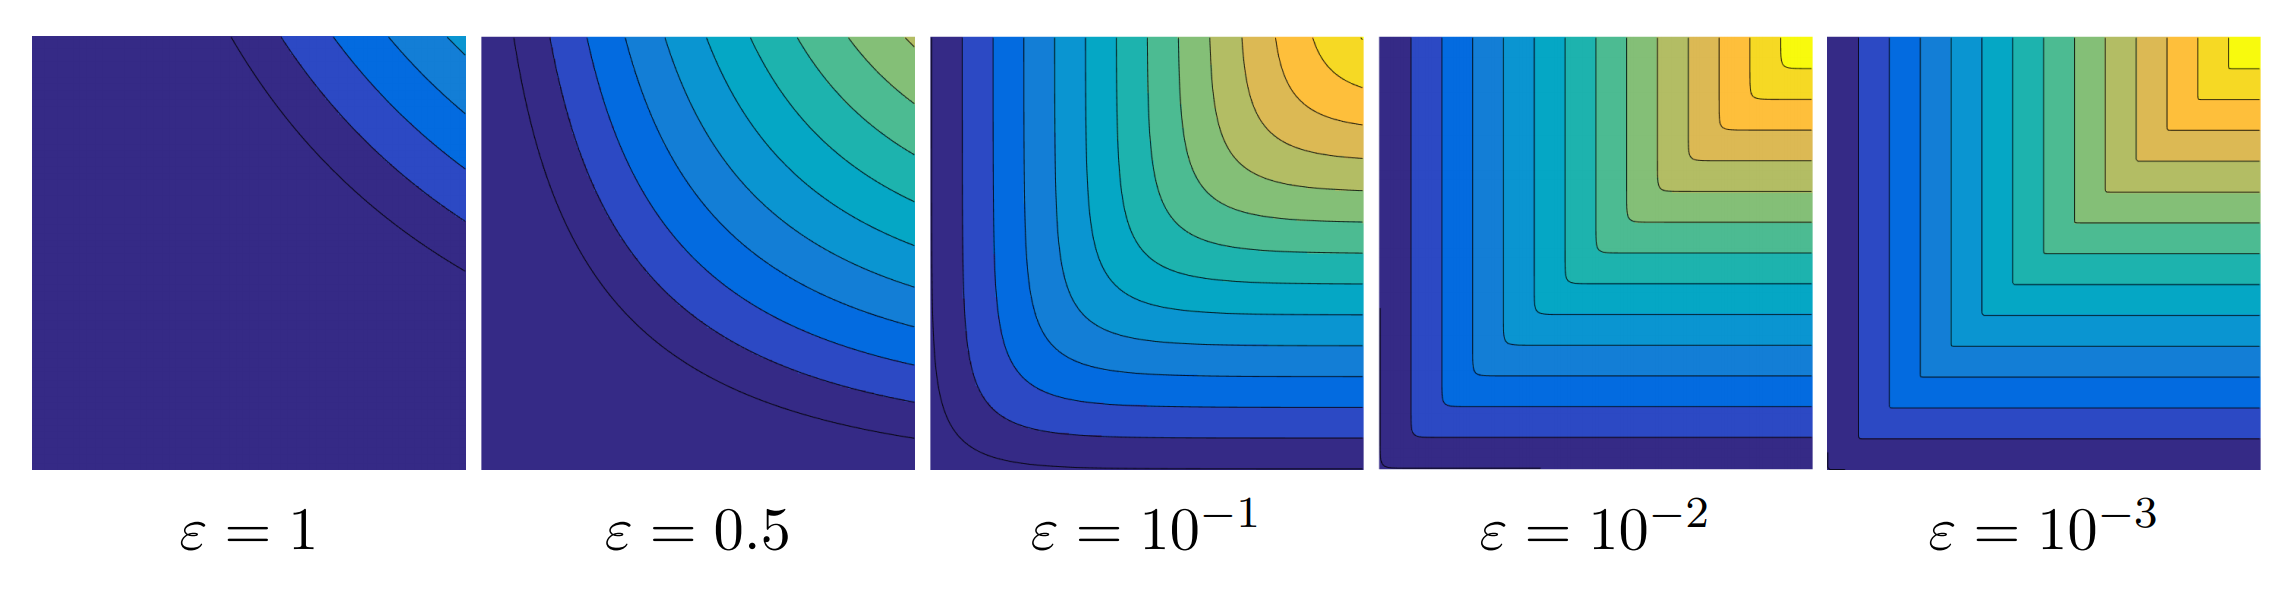
\includegraphics[width=0.9\linewidth]{img/min_eps}
  \label{fig:ot}
  \caption{Soft-minimum}
\end{figure}

Using this notation,

\begin{equation}
  \begin{array}{l}
    {\left(\mathbf{f}^{(\ell+1)}\right)_{i}=\min _{\varepsilon}\left(\mathbf{C}_{i j}-\mathbf{g}_{j}^{(\ell)}\right)_{j}+\varepsilon \log \mathbf{\mu}_{i}} \\
    {\left(\mathbf{g}^{(\ell+1)}\right)_{j}=\min _{\varepsilon}\left(\mathbf{C}_{i j}-\mathbf{f}_{i}^{(\ell)}\right)_{i}+\varepsilon \log \mathbf{\nu}_{j}}
    \end{array}
\end{equation}

To simplify notations, we introduce an operator that
takes a matrix as input and outputs now a column vector of the soft-minimum values
of its columns or rows. Namely, for any matrix $\mathbf{A} \in \mathbb{R}^{m \times n}$, we define

\begin{equation}
  \begin{array}{l}
    {\operatorname{Min}_{\varepsilon}^{\mathrm{row}}(\mathbf{A}) \stackrel{\text { def. }}{=}\left(\min _{\varepsilon}\left(\mathbf{\mu}_{i, j}\right)_{j}\right)_{i} \in \mathbb{R}^{m}} \\
    {\operatorname{Min}_{\varepsilon}^{\mathrm{col}}(\mathbf{A}) \stackrel{\mathrm{def}}{=}\left(\min _{\varepsilon}\left(\mathbf{\nu}_{i, j}\right)_{i}\right)_{j} \in \mathbb{R}^{n}}
    \end{array}
\end{equation}

Using this notation, Sinkhorn's iterates read

\begin{equation}
  \begin{array}{l}
    {\mathbf{f}^{(\ell+1)}=\operatorname{Min}_{\varepsilon}^{\mathrm{row}}\left(\mathbf{C}-\mathbf{1}_{m} \mathbf{g}^{(\ell)^{\mathrm{T}}}\right)+\varepsilon \log \mathbf{\mu}} \\
    {\mathbf{g}^{(\ell+1)}=\operatorname{Min}_{\varepsilon}^{\mathrm{col}}\left(\mathbf{C}-\mathbf{f}^{(\ell)} \mathbf{1}_{n}^{\mathrm{T}}\right)+\varepsilon \log \mathbf{\nu}}
    \end{array}
\end{equation}

While mathematically equivalent to the Sinkhorn
updates \ref{eq:sinkhorn}, iterations above suggest using the log-sum-exp stabilization
trick to avoid underflow for small values of $\epsilon$. Writing $\underline{z}=\min \mathbf{z}$, that trick suggests
evaluating $\min_{\varepsilon} z$ as

\begin{equation}
  \operatorname{min}_{\varepsilon} \mathbf{z}=\underline{z}-\varepsilon \log \sum e^{-\left(\mathbf{z}_{i}-\underline{Z}\right) / \varepsilon}
\end{equation}

Instead of substracting $\mathbf{z}$ to stabilize the log-domain iterations as above, one can actually substract the previously computed scalings. This leads to the stabilized iteration

\begin{equation}
  \begin{array}{l}
    {\mathbf{f}^{(\ell+1)}=\operatorname{Min}_{\varepsilon}^{\mathrm{row}}\left(\mathbf{S}\left(\mathbf{f}^{(\ell)}, \mathbf{g}^{(\ell)}\right)\right)-\mathbf{f}^{(\ell)}+\varepsilon \log (\mathbf{\mu})} \\
    {\mathbf{g}^{(\ell+1)}=\operatorname{Min}_{\varepsilon}^{\mathrm{col}}\left(\mathbf{S}\left(\mathbf{f}^{(\ell+1)}, \mathbf{g}^{(\ell)}\right)\right)-\mathbf{g}^{(\ell)}+\varepsilon \log (\mathbf{\nu})}
    \end{array}
\end{equation}

where we defined 

\begin{equation}
  \mathbf{S}(\mathbf{f}, \mathbf{g})=\left(\mathbf{C}_{i, j}-\mathbf{f}_{i}-\mathbf{g}_{j}\right)_{i, j}
\end{equation}

In contrast to the original iterations \ref{eq:sinkhorn}, these log-domain iterations
are stable for arbitrary $\epsilon$, because the quantity $\mathbf{S}(\mathbf{f}, \mathbf{g})$ stays bounded during the
iterations. The downside is that it requires nm computations of exp at each step. Computing a $\mathrm{Min}_{\varepsilon}^{\mathrm{row}}$ is typically substantially slower than matrix multiplications
and requires computing line by line soft-minima of matrices $\mathbf{S}$. There is therefore no
efficient way to parallelize the application of Sinkhorn maps for several marginals simultaneously. In Euclidean domains of small dimension, it is possible to develop efficient
multiscale solvers with a decaying $\epsilon$ strategy to significantly speed up the computation
using sparse grids.

\vspace{2ex}
    \begin{algorithm}[htbp]
        \SetAlgoNoLine
        \caption{Block Coordinate Ascent algorithm for regularized problem} 
        \KwIn{parameters $\mu$, $\nu$, $c$}
        \KwIn{epsilon $\epsilon$}
        Initialize variables $\mathbf{f}, \mathbf{g} = \boldsymbol{1}$\\
        Initialize  $\mathbf{K} = \exp^{-c/\epsilon}$\\
        \While{ stopping criterion not met } 
        {  
          Update $\mathbf{S}$: $\mathbf{S}(\mathbf{f}, \mathbf{g})=\left(\mathbf{C}_{i, j}-\mathbf{f}_{i}-\mathbf{g}_{j}\right)_{i, j}$\\
          Update $\mathbf{f}$: ${\mathbf{f}^{(\ell+1)}=\operatorname{Min}_{\varepsilon}^{\mathrm{row}}\left(\mathbf{S}\left(\mathbf{f}^{(\ell)}, \mathbf{g}^{(\ell)}\right)\right)-\mathbf{f}^{(\ell)}+\varepsilon \log (\mathbf{\mu})}$\\
          Update $\mathbf{S}$: $\mathbf{S}(\mathbf{f}, \mathbf{g})=\left(\mathbf{C}_{i, j}-\mathbf{f}_{i}-\mathbf{g}_{j}\right)_{i, j}$\\
          Update $\mathbf{g}$: ${\mathbf{g}^{(\ell+1)}=\operatorname{Min}_{\varepsilon}^{\mathrm{col}}\left(\mathbf{S}\left(\mathbf{f}^{(\ell+1)}, \mathbf{g}^{(\ell)}\right)\right)-\mathbf{g}^{(\ell)}+\varepsilon \log (\mathbf{\nu})}$\\
        }
        Calculate $\mathbf{u} = \exp(\mathbf{f}/\epsilon)$\\
        Calculate $\mathbf{v} = \exp(\mathbf{g}/\epsilon)$\\
        Calculate $\mathbf{P} = (\operatorname{diag}{\mathbf{u}}) \mathbf{K} (\operatorname{diag}{\mathbf{v}})$\\
    \end{algorithm}


%%%   Section 5: Numerical Results  %%%
% Section 5: Numerical Results

\section{Numerical Results}


\subsection{Datasets}
In orde to compare the performance of different algorithms, we used three types of datasets to test algorithms discussed above, including artificial generated datasets and real images. In short, we have three different types of datasets:
\begin{itemize}
    \item Random Generated Dataset
    \item Ellipse and Caffarelli Dataset [5]
    \item DOTmark Dataset [6]
\end{itemize}

We assume that the cost of transporting a unit mass from $x \in X \subset \mathbb{R}^2$ to $y \in Y \subset \mathbb{R}^2$ is $c_p(x,y) = \|x-y\|^p$ for some $p \geq 1$. The minimum cost for transferring $\mu$ to $\nu$ is then given by 

\begin{equation}
    C_p (\mu, \nu) = \min_{x \in \Pi(\mu,\nu)} \|x-y\|^p d\pi(x,y)
\end{equation}

For realistic considerations, we use $\mathbf{L}_2$ distance as our metrics.
  
Random generated samples consists of uniform samples on $[-1, 1]^2$ of size $n$, weights $\mu$ and $\nu$ are uniformly 
sampled on $[-1,1]^2$ and normalized with $\sum_i \mu_i = 1$, $\sum_j \nu_j = 1$.

The ellipse example consists of two uniform samples (source and target data set) of size $n$ from the unit circle
with normal distributed noise added with zero mean and standard deviation $0.1$. The source
data sample is then scaled in the x-Axis by $1.3$ and in the y-Axis by $0.9$, while the target
data set is scaled in the x-Axis by $0.9$ and in the y-Axis by $1.1$.

\begin{figure}[htbp]
    \centering
    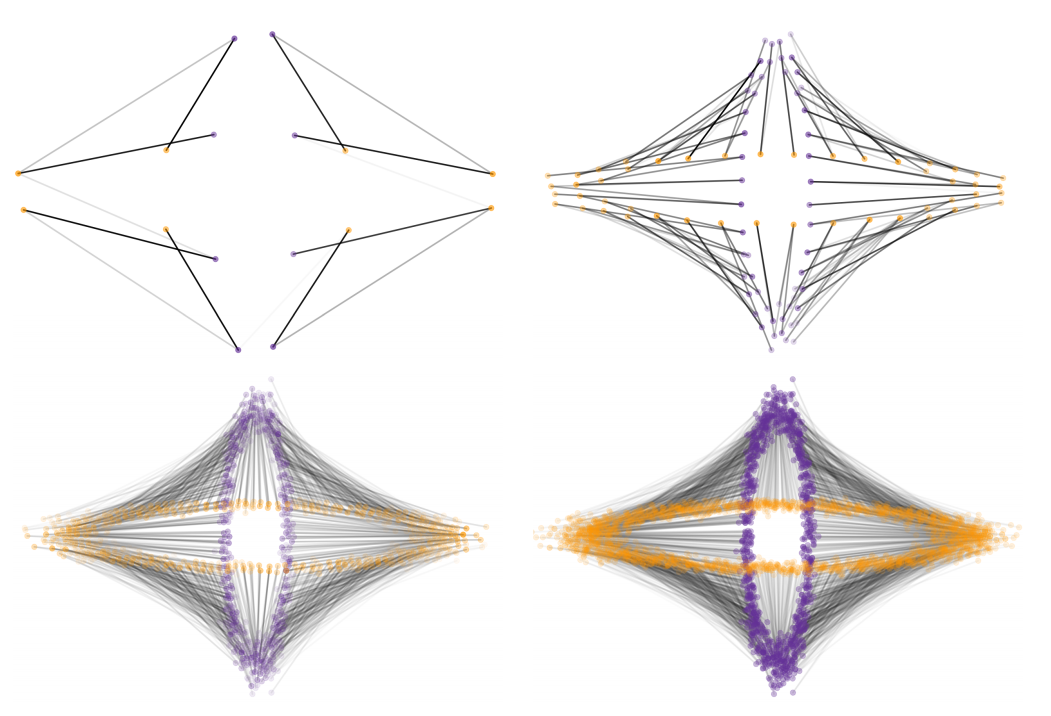
\includegraphics[width=0.6\linewidth]{img/ellipse}
    \label{fig:ot}
    \caption{Illustration of Optimal Transport on Ellipse dataset with different coarsen level}
  \end{figure}

Caffarelli's example consists of two uniform samples on $[-1, 1]^2$ of size $n$. Any points outside the unit circle are then
discarded. Additionally, the target data sample is split along the x-Axis at $0$ and shifted by
$+2$ and $-2$ for points with positive and negative x-Axis values, respectively.

\begin{figure}[htbp]
    \centering
    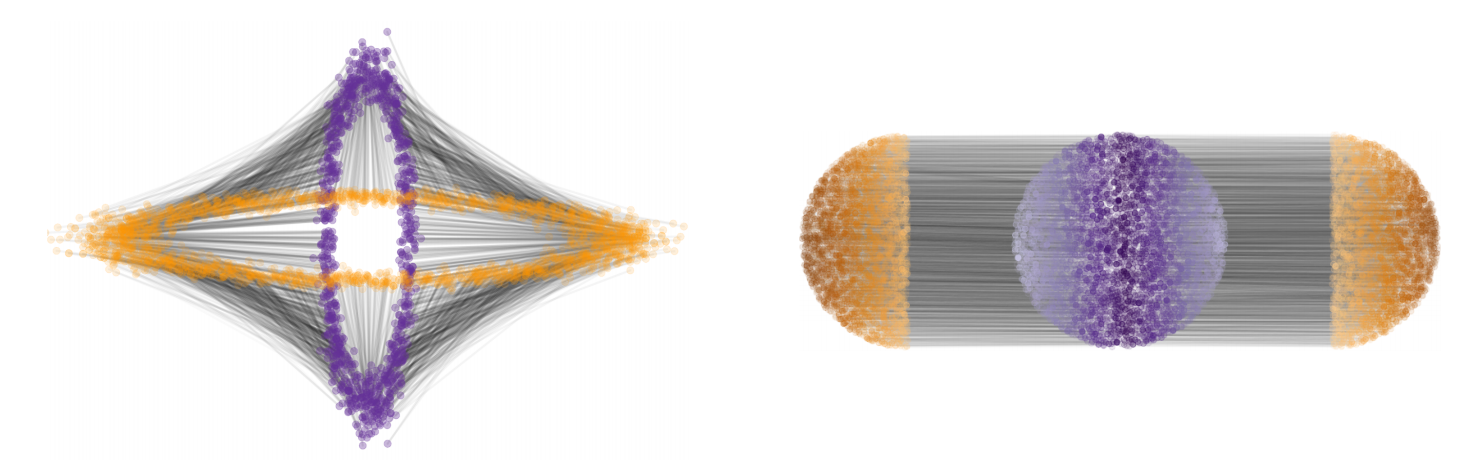
\includegraphics[width=0.6\linewidth]{img/ellipse_caffa}
    \label{fig:ot}
    \caption{Illustration of Optimal Transport on Ellipse dataset and Caffarelli dataset}
  \end{figure}

The DOT benchmark [6] consists of 10 classes of 10 different images, each of which is available at the 5 different
resolutions from $a \times a  = 32 \times 32$ to $512 \times 512$. In computation, each data point is $m = n = a^2$.  This allows
for a total of 45 computations of Wasserstein distances between two images for any one class at any fixed resolution. for convenience, we used the $32 \times 32$ and $64 \times 64$ smaples for experiments.

Table 1 gives an overview of how the classes were created.
Classes 1-7 are random simulations of scenarios based on various probability distributions.
Images at different resolutions are generated independently from each other but according to the same laws.
Classes 8-10 were obtained by ad-hoc choices of simple geometric shapes, classic test images and images of mitochondria acquired using STED
super-resolution microscopy. For geometric shapes and classic test images
the various resolutions available are coarsenings of a single image. For the microscopy
images different clippings of various sizes have been selected from larger images to obtain
the various resolutions.

\vspace{5ex}
\begin{table}[htbp]
	\caption{DOTmark datasent}
	\centering
	\begin{tabular}[width=1.0\linewidth]{lll}
		\toprule
		\quad  & Dataset & Description\\
    \midrule
            1  & WhiteNoise    & i.i.d. uniformly distributed values in [0, 1] at each pixel\\
            2  & GRFrough      & GRF with $\sigma = 1$, $\nu = 0.25$, $\gamma = 0.5$\\
            3  & GRFmoderate   & GRF with $\sigma = 1$, $\nu = 2.5$, $\gamma = 0.15$\\
            4  & GRFsmooth     & GRF with $\sigma = 1$, $\nu = 2.5$, $\gamma = 0.3$\\
            5  & LogGRF        & exp-function of a GRF with $\sigma = 1$, $\nu = 0.5$, $\gamma = 0.4$\\
            6  & CauchyDensity & Bivariate Cauchy density with random center and a varying scale ellipse\\
            7  & LogitGRF      & Logistic function of a GRF with $\sigma = 4$, $\nu = 4.5$, $\gamma = 0.1$\\
            8  & Shapes        & An ad-hoc choice of simple geometric shapes\\
            9  & ClassicImages & Standard grayscale test images used in image processing\\
            10 & Microscopy    & Clippings from STED microscopy images of mitochondria\\
        \bottomrule
	\end{tabular}
	\label{tab:tabledot}
\end{table}

\begin{figure}[htbp]
    \centering
    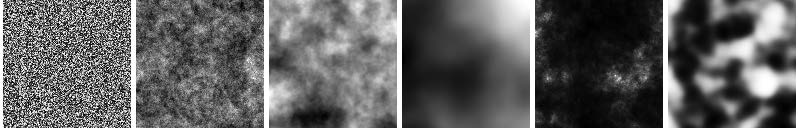
\includegraphics[width=0.9\linewidth]{img/dot_1to6}
    \label{fig:ot}
    \caption{The images in the classes 1-6 at resolution 128 $\times$ 128}
\end{figure}

\begin{figure}[htbp]
    \centering
    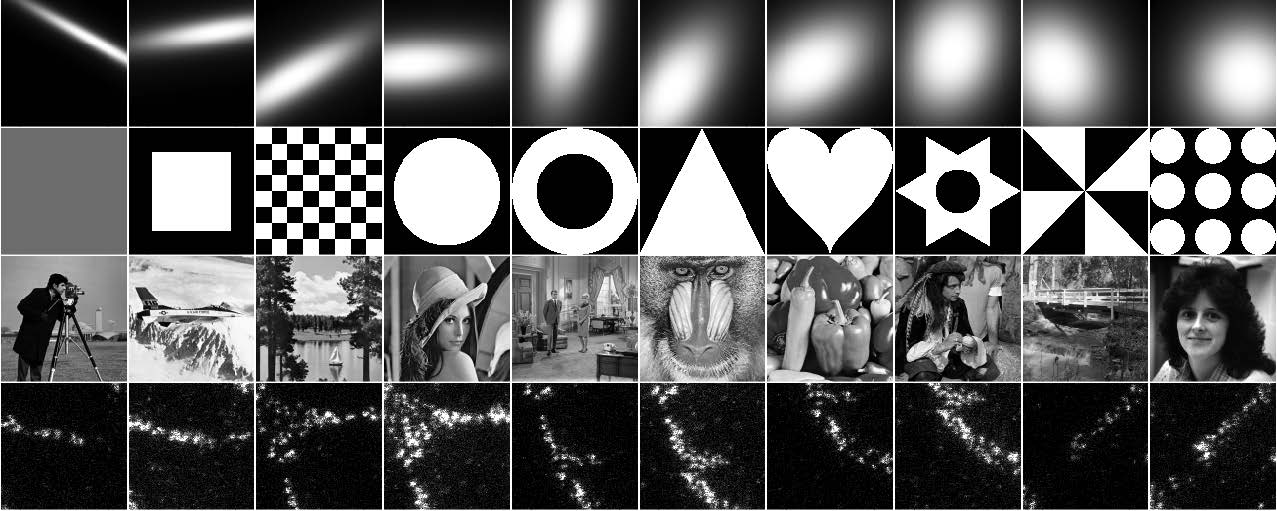
\includegraphics[width=0.9\linewidth]{img/dot_7to10}
    \label{fig:ot}
    \caption{The images in the classes 7-10 at resolution 128 $\times$ 128}
\end{figure}

\clearpage
\subsection{Numercial Results and Intepretations}

We use three main metrics to evaluate all of these algorithms:

\begin{itemize}
    \item Running time
    \item Function value
    \item Constraints $\mu$ and $\nu$ 
\end{itemize}

To measure the satisfaction of constraints, $\mathbf{L}_1$ norm of $\mathbf{\mu} - \mathbf{\pi}_{i\cdot}$ and $\mathbf{\nu} - \mathbf{\pi}_{\cdot j}$ was introduced. On the consideration of time consuming, we conduct our experiments with size $m = n = 64, 128, 256, 512, 1024, 2048$.

Obviously, the running time is an important metrics to measure different algorithms under different test data. In addition, object value can also shows performance of different algorithms, though for entropy regularized methods such as sinkhorn algorithm the function value has been modified with regularization term and then can not be use for comparison.
However, the distance between the suboptimal tranport variable $\pi$ and the optimal transport variable $\tilde \pi$ does not reflect the merits of the algorithm, because it depends on the nature of the cost matrix $\mathbf{C}$. Consider the following example:

\begin{equation}
    \begin{array}{cl}
        {\min } & {\mathbf{t} \mathbf{r}\left(\left(\begin{array}{cc}
        {1+\epsilon} & {1 + \frac{\epsilon}{2}}\\
        {1} & {1} \\
        \end{array}\right)\left(\begin{array}{cc}
        {\pi_{11}} & {\pi_{12}} \\
        {\pi_{21}} & {\pi_{22}}
        \end{array}\right)\right.} \\
        {\text { s.t. }} & {\pi_{11}+\pi_{12}=1} \\
        & {\pi_{21}+\pi_{22}=1} \\
        & {\pi_{11}+\pi_{21}=1} \\
        & {\pi_{12}+\pi_{22}=1}
    \end{array}
\end{equation}

Then the difference between the object value of the optimal solution $\tilde \pi_{ij} = \left(\begin{array}{ll}{0} & {1} \\{1} & {0}\end{array}\right)$ and the suboptimal solution $\pi = \left(\begin{array}{ll}{1} & {0} \\{0} & {1}\end{array}\right)$ is less than $\epsilon$, but the distance after the two are transformed into a vector is significantly larger than $\epsilon$.

Tables below show our experiments results, more detailed data can be found in \textbf{/code/results} folder.

\begin{table}[htbp]
	\caption{Results of Raw Mosek solver and Raw Gurobi solver on Random Generated Dataset}
	\centering
    \begin{tabular}{|c|c|llllll|}
    \hline
    $m = n$             &          & Mosek primal & Mosek dual  & Mosek interior & Gurobi primal & Gurobi dual & Gurobi interior\\
    \hline
    \multirow{4}*{64}   &err $\mu$ & 1.73472e-17  & 1.56125e-17 & 6.99572e-11    & 1.56125e-17   & 1.90820e-17 & 1.56125e-17    \\   
                        &err $\nu$ & 1.73472e-16  & 1.68268e-16 & 6.05657e-11    & 1.56125e-16   & 1.58727e-16 & 1.54390e-16    \\  
                        &fval      & 2.07168e-02  & 2.07168e-02 & 2.07168e-02    & 2.07168e-02   & 2.07168e-02 & 2.07168e-02    \\
                        &time      & 3.12448e-02  & 3.47526e-02 & 3.42710e-02    & 4.78537e-02   & 4.80292e-02 & 7.72452e-02    \\
    \hline
    \multirow{4}*{128}  &err $\mu$ & 7.38910e-06  & 1.04083e-17 & 6.21169e-12    & 3.46945e-18   & 3.46945e-18 & 5.20417e-18    \\   
                        &err $\nu$ & 7.38910e-06  & 1.14275e-16 & 6.21459e-12    & 1.18395e-16   & 1.18395e-16 & 1.17934e-16    \\  
                        &fval      & 1.85776e-02  & 1.85775e-02 & 1.85775e-02    & 1.85775e-02   & 1.85775e-02 & 1.85775e-02    \\
                        &time      & 8.82461e-02  & 1.05152e-01 & 3.42710e-02    & 2.18717e-01   & 2.67161e-01 & 3.70859e-01    \\
    \hline
    \multirow{4}*{256}  &err $\mu$ & 1.75611e-05  & 3.62395e-17 & 8.84693e-11    & 1.04083e-17   & 1.12757e-17 & 1.12757e-17    \\   
                        &err $\nu$ & 1.75611e-05  & 3.43123e-16 & 8.84696e-11    & 3.23526e-16   & 3.23526e-16 & 3.23960e-16    \\  
                        &fval      & 9.37655e-03  & 9.37637e-03 & 9.37637e-03    & 9.37637e-03   & 9.37637e-03 & 9.37637e-03    \\
                        &time      & 3.19547e-01  & 4.38276e-01 & 5.48973e-01    & 1.01217e+00   & 1.12126e+00 & 1.07492e+00    \\
    \hline
    \multirow{4}*{512}  &err $\mu$ & 4.29996e-05  & 5.06695e-17 & 1.13676e-10    & 8.48388e-18   & 3.10109e-16 & 1.12757e-17    \\   
                        &err $\nu$ & 4.29996e-05  & 3.38688e-16 & 1.13677e-10    & 8.48388e-18   & 1.25767e-17 & 3.23960e-16    \\  
                        &fval      & 4.30472e-03  & 4.30454e-03 & 4.30454e-03    & 4.30454e-03   & 4.30454e-03 & 9.37637e-03    \\
                        &time      & 1.42172e+00  & 2.23522e+00 & 2.73145e+00    & 3.47143e+00   & 3.77973e+00 & 1.07492e+00    \\
    \hline    
    \multirow{4}*{1024} &err $\mu$ & 1.06018e-04  & 1.47138e-16 & 1.01099e-13    & 1.09504e-17   & 3.64400e-16 & 1.20346e-17    \\   
                        &err $\nu$ & 1.06018e-04  & 5.08930e-16 & 1.00871e-13    & 3.64753e-16   & 1.15196e-17 & 3.65837e-16    \\  
                        &fval      & 1.94602e-03  & 1.94578e-03 & 1.94578e-03    & 1.94578e-03   & 1.94578e-03 & 1.94578e-03   \\
                        &time      & 6.45907e+00  & 1.37058e+01 & 1.33225e+01    & 1.73826e+01   & 1.31655e+01 & 1.73745e+01    \\
    \hline
    \multirow{4}*{2048} &err $\mu$ & 2.65157e-04  & 1.12464e-16 & 5.64365e-11    & 1.20889e-17   & 9.78113e-16 & 1.13841e-17    \\   
                        &err $\nu$ & 2.65157e-04  & 1.08728e-15 & 5.36207e-11    & 9.76758e-16   & 9.18861e-18 & 9.75701e-16    \\  
                        &fval      & 1.50347e-03  & 1.50297e-03 & 1.50297e-03    & 1.50297e-03   & 1.50297e-03 & 1.50297e-03   \\
                        &time      & 3.59507e+01  & 1.28866e+02 & 6.74333e+01    & 3.16742e+01   & 5.92715e+01 & 9.67955e+01    \\
    \hline   
    \end{tabular}
    \label{tab:table1}
\end{table}

It seems that Gurobi can always reach the real optimal solution, and MOSEK sometimes fails. For MOSEK,
 the simplex method on primal problem is faster than the interior method and dual simplex method. For Gurobi, the simplex method is usually faster than the interior method. As one of the most famous algorithms in 20th century, simplex method was designed for solving linear programming problems. Poor performance of dual simplex may be caused by a large number of constraints. In summary, Gurobi has better performance that MOSEK.

\begin{table}[htbp]
	\caption{Results of ADMM, Sinkhorn and BlockCA algorithm on Random Generated Dataset}
	\centering
    \begin{tabular}{|c|c|lllll|}
    \hline
    $m = n$             &          & Gurobi primal & ADMM primal & ADMM dual   & Sinkhorn    & BlockCA    \\
    \hline
    \multirow{4}*{64}   &err $\mu$ & 1.56125e-17   & 1.40712e-05 & 6.50195e-01 & 1.00180e-16 & 5.41017e-16\\   
                        &err $\nu$ & 1.56125e-16   & 1.41582e-05 & 6.27594e-01 & 1.90874e-16 & 3.94243e-16\\  
                        &fval      & 2.07168e-02   & 2.07460e-02 & 8.77846e-04 & 2.73941e-02 & 2.73941e-02\\
                        &time      & 4.78537e-02   & 1.22792e+00 & 1.38214e+00 & 8.93044e-03 & 1.44658e-01\\
    \hline
    \multirow{4}*{128}  &err $\mu$ & 3.46945e-18   & 4.72795e-05 & 8.45667e-01 & 1.39456e-16 & 5.54624e-16\\   
                        &err $\nu$ & 1.18395e-16   & 4.64422e-05 & 8.56649e-01 & 2.61211e-16 & 5.22084e-16\\  
                        &fval      & 1.85775e-02   & 1.85941e-02 & 8.22017e-05 & 2.92237e-02 & 2.92237e-02\\
                        &time      & 2.67161e-01   & 4.53466e+00 & 3.89032e+00 & 6.39679e-02 & 4.98657e-01\\
    \hline
    \multirow{4}*{256}  &err $\mu$ & 1.04083e-17   & 4.96761e-05 & 9.04781e-01 & 3.11044e-16 & 6.12256e-16\\  
                        &err $\nu$ & 3.23526e-16   & 5.02865e-05 & 9.00866e-01 & 3.62530e-16 & 5.78530e-16\\ 
                        &fval      & 9.37637e-03   & 9.38144e-03 & 1.20866e-05 & 2.88136e-02 & 2.88136e-02\\
                        &time      & 1.01217e+00   & 1.81699e+01 & 8.70793e+00 & 8.24754e-02 & 2.26562e+00\\
    \hline
    \multirow{4}*{512}  &err $\mu$ & 8.48388e-18   & 1.31110e-04 & 9.53515e-01 & 3.42523e-16 & 6.55963e-16\\   
                        &err $\nu$ & 8.48388e-18   & 1.33937e-04 & 9.53115e-01 & 5.30280e-16 & 7.73707e-16\\  
                        &fval      & 4.30454e-03   & 4.30575e-03 & 1.35802e-06 & 2.81078e-02 & 2.81078e-02\\
                        &time      & 3.47143e+00   & 7.43271e+01 & 6.13705e+01 & 2.81078e-01 & 1.08770e+01\\
    \hline    
    \multirow{4}*{1024} &err $\mu$ & 1.09504e-17   & 2.73918e-04 & 9.72007e-01 & 3.86662e-16 & 6.89612e-16\\   
                        &err $\nu$ & 3.64753e-16   & 2.74108e-04 & 9.72809e-01 & 7.61287e-16 & 1.02598e-15\\ 
                        &fval      & 1.94578e-03   & 1.94916e-03 & 2.51372e-07 & 2.79386e-03 & 2.79386e-02\\
                        &time      & 1.73826e+01   & 3.67489e+02 & 2.08239e+02 & 1.02975e+00 & 3.62734e+01\\
    \hline
    \multirow{4}*{2048} &err $\mu$ & 1.20889e-17   & 1.01361e-03 & 9.88752e-01 & 9.68066e-16 & 1.09343e-15\\   
                        &err $\nu$ & 9.76758e-16   & 1.02573e-03 & 9.89591e-01 & 1.09554e-15 & 1.53059e-15\\  
                        &fval      & 1.50297e-03   & 1.49998e-03 & 2.11058e-08 & 2.76252e-03 & 2.76252e-02\\
                        &time      & 3.16742e+01   & 5.71285e+03 & 3.14300e+03 & 8.98797e+00 & 4.12741e+02\\
    \hline
    \end{tabular}
    \label{tab:table1}
\end{table}

Generally speaking, The ADMM method does not have good performance. On the one hand, the error term is large, which is because the equality constraint is difficult to achieve. On the other hand, the required time is much longer than the general algorithm of Mosek and Gurobi. This is because the algorithm will stay at $\pi = \frac{1}{m n}$ for a long time, and it will not start the convergence step until some variables start to increase significantly. what's more, ADMM method is a first order method which means it has slow convergence rate.

As mentioned before, in practice, the Sinkhorn algorithm suffers from numerical overflow when the regularization parameter $\epsilon$ is small compared to the entries of the cost
matrix $\mathbf{C}$. This concern can be alleviated to some extent by carrying out computations
in the log domain. Here Block Coordinate Ascent algorithm was introduced. From the experiments we can see that entropy regularized methods applied with Sinkhorn algorithm and Block Coordinate Ascent algorithm convergence very fast with the slightest violation with all the constraints of $\mu$ and $\nu$ corresponding to err $\mu$ and err $\nu$ shown.

 \begin{table}[htbp]
	\caption{Results of Raw Mosek solver and Raw Gurobi solver on DOTmark Dataset}
	\centering
    \begin{tabular}{|c|c|llllll|}
    \hline
    Class                   &          & Mosek primal & Mosek dual  & Mosek interior & Gurobi primal & Gurobi dual & Gurobi interior\\
    \hline
    \multirow{4}*{WNoise}   &err $\mu$ & 1.04105e-04  & 1.43060e-16 & 2.60955e-11    & 0.00000e+00   & 0.00000e+00 & 0.00000e+00    \\   
                            &err $\nu$ & 1.04106e-04  & 6.93859e-10 & 7.19976e-10    & 6.93859e-10   & 6.93859e-10 & 6.93859e-10    \\  
                            &fval      & 6.49762e-04  & 6.49817e-04 & 6.49817e-04    & 6.49817e-04   & 6.49817e-04 & 6.49817e-04    \\
                            &time      & 6.37157e+00  & 1.00645e+01 & 1.09153e+01    & 1.96804e+01   & 1.80495e+01 & 2.56732e+01    \\
    \hline
    \multirow{4}*{GRFrough} &err $\mu$ & 9.86331e-05  & 2.14455e-16 & 3.88285e-14    & 0.00000e+00   & 0.00000e+00 & 0.00000e+00    \\   
                            &err $\nu$ & 9.86322e-05  & 8.99345e-10 & 8.99386e-10    & 8.99345e-10   & 8.99345e-10 & 8.99345e-10    \\  
                            &fval      & 1.24126e-03  & 1.24131e-03 & 1.24131e-03    & 1.24131e-03   & 1.24131e-03 & 1.24131e-03    \\
                            &time      & 6.22112e+00  & 1.60985e+01 & 1.20426e+01    & 1.70455e+01   & 1.44343e+01 & 2.98131e+01    \\
    \hline
    \multirow{4}*{GRFmid}   &err $\mu$ & 9.82285e-05  & 1.81604e-16 & 5.15640e-11    & 0.00000e+00   & 5.89424e-10 & 5.89424e-10    \\   
                            &err $\nu$ & 9.82291e-05  & 5.89424e-10 & 7.33106e-10    & 5.89424e-10   & 0.00000e+00 & 0.00000e+00    \\  
                            &fval      & 1.29959e-02  & 1.29962e-02 & 1.29962e-02    & 1.29962e-02   & 1.29962e-02 & 1.29962e-02    \\
                            &time      & 7.08524e+00  & 3.11953e+01 & 1.08397e+01    & 1.62867e+01   & 1.74454e+01 & 2.98980e+01    \\
    \hline
    \multirow{4}*{GRFmid2}  &err $\mu$ & 9.78652e-05  & 1.96051e-16 & 2.27771e-12    & 0.00000e+00   & 4.81123e-10 & 4.81123e-10    \\   
                            &err $\nu$ & 9.78657e-05  & 4.81123e-10 & 4.83410e-10    & 4.81123e-10   & 0.00000e+00 & 0.00000e+00    \\  
                            &fval      & 7.01347e-03  & 7.01329e-03 & 7.01329e-03    & 7.01329e-03   & 7.01329e-03 & 7.01329e-03    \\
                            &time      & 8.29048e+00  & 2.58863e+01 & 1.16190e+01    & 1.54850e+01   & 1.46085e+01 & 1.82575e+01    \\
    \hline    
    \multirow{4}*{LogGRF}   &err $\mu$ & 9.79684e-05  & 1.74543e-16 & 1.41349e-13    & 0.00000e+00   & 0.00000e+00 & 0.00000e+00    \\   
                            &err $\nu$ & 9.79684e-05  & 3.44473e-11 & 3.45826e-11    & 3.44471e-11   & 3.44471e-11 & 3.44471e-11    \\  
                            &fval      & 1.14762e-02  & 1.14762e-02 & 1.14762e-02    & 3.44471e-11   & 1.14762e-02 & 1.14762e-02    \\
                            &time      & 6.61064e+00  & 2.25776e+01 & 1.25897e+01    & 1.46135e+01   & 1.81754e+01 & 2.23398e+01    \\
    \hline
    \multirow{4}*{Cauchy}   &err $\mu$ & 8.95380e-05  & 1.69054e-16 & 4.53139e-11    & 0.00000e+00   & 6.45741e-10 & 6.45741e-10    \\   
                            &err $\nu$ & 8.95387e-05  & 6.45741e-10 & 5.36207e-11    & 6.45741e-10   & 0.00000e+00 & 0.00000e+00    \\  
                            &fval      & 2.70715e-02  & 2.70716e-02 & 2.70716e-02    & 2.70716e-02   & 2.70716e-02 & 2.70716e-02    \\
                            &time      & 6.27543e+00  & 3.43761e+01 & 1.25938e+01    & 1.41227e+01   & 1.66956e+01 & 4.97750e+01    \\
    \hline   
    \multirow{4}*{LogitGRF} &err $\mu$ & 1.04014e-04  & 1.61844e-16 & 6.22315e-10    & 0.00000e+00   & 1.23453e-09 & 1.23453e-09    \\   
                            &err $\nu$ & 1.04013e-04  & 1.23453e-09 & 1.83005e-09    & 1.23453e-09   & 0.00000e+00 & 0.00000e+00    \\  
                            &fval      & 1.90306e-02  & 1.90301e-02 & 1.90301e-02    & 1.90301e-02   & 1.90301e-02 & 1.90301e-02    \\
                            &time      & 6.59682e+00  & 2.55476e+01 & 1.09550e+01    & 1.51339e+01   & 1.87915e+01 & 3.24828e+01    \\
    \hline
    \multirow{4}*{Shape}    &err $\mu$ & 3.10808e-05  & 6.51926e-09 & 1.54226e-08    & 0.00000e+00   & 6.51926e-09 & 6.51926e-09    \\   
                            &err $\nu$ & 3.10743e-05  & 4.77049e-17 & 1.07581e-08    & 6.51926e-09   & 0.00000e+00 & 0.00000e+00    \\  
                            &fval      & 6.00170e-03  & 6.00148e-03 & 6.00148e-03    & 6.00148e-03   & 6.00148e-03 & 6.00148e-03    \\
                            &time      & 2.45428e+00  & 4.44892e+00 & 2.97079e+00    & 1.17216e+01   & 1.16747e+01 & 1.31421e+01    \\
    \hline
    \multirow{4}*{Classic}  &err $\mu$ & 9.68013e-05  & 1.20292e-16 & 8.39560e-12    & 0.00000e+00   & 2.61934e-10 & 2.61934e-10    \\   
                            &err $\nu$ & 9.68016e-05  & 2.61935e-10 & 2.70569e-10    & 2.61934e-10   & 0.00000e+00 & 0.00000e+00    \\  
                            &fval      & 2.13840e-03  & 2.13855e-03 & 2.13855e-03    & 2.13855e-03   & 2.13855e-03 & 2.13855e-03    \\
                            &time      & 7.26325e+00  & 1.91323e+01 & 1.30328e+01    & 1.54186e+01   & 1.40239e+01 & 2.08600e+01    \\
    \hline
    \multirow{4}*{Micro}    &err $\mu$ & 9.11961e-05  & 1.09938e-16 & 1.40660e-10    & 0.00000e+00   & 0.00000e+00 & 0.00000e+00   \\   
                            &err $\nu$ & 9.11973e-05  & 1.25146e-09 & 1.24353e-09    & 1.25146e-09   & 1.25146e-09 & 1.25146e-09    \\  
                            &fval      & 5.60394e-02  & 5.60383e-02 & 5.60383e-02    & 5.60383e-02   & 5.60383e-02 & 5.60383e-02    \\
                            &time      & 5.27145e+00  & 2.11592e+01 & 9.32959e+00    & 1.44868e+01   & 1.58690e+01 & 1.78717e+02    \\
    \hline
    \end{tabular}
    \label{tab:table1}
\end{table}



\begin{table}[htbp]
	\caption{Results of ADMM, Sinkhorn and BlockCA algorithm on DOTmark Dataset}
	\centering
    \begin{tabular}{|c|c|lllll|}
    \hline
    Class                   &          & Gurobi primal & ADMM primal & ADMM dual  & Sinkhorn   & BlockCA    \\
    \hline
    \multirow{4}*{WNoise}   &err $\mu$ & 0.00000e+00   & 1.28341e-04  & 3.33216e-01 & 6.93859e-10 & 1.24606e-07 \\   
                            &err $\nu$ & 6.93859e-10   & 1.16042e-04  & 3.33214e-01 & 7.56495e-16 & 1.27072e-07 \\  
                            &fval      & 6.49817e-04   & 6.49518e-04  & 0.00000e+00 & 2.76750e-03 & 2.76750e-02 \\
                            &time      & 1.96804e+01   & 2.05072e+02  & 1.76776e+02 & 4.96325e-01 & 4.06536e+01 \\
    \hline
    \multirow{4}*{GRFrough} &err $\mu$ & 0.00000e+00   & 1.36891e-04  & 2.13545e-01 & 8.99345e-10 & 1.23457e-07 \\   
                            &err $\nu$ & 8.99345e-10   & 1.35197e-04  & 2.13544e-01 & 7.54279e-16 & 1.22399e-07 \\  
                            &fval      & 1.24131e-03   & 1.24030e-03  & 0.00000e+00 & 2.77295e-02 & 2.77295e-01 \\ 
                            &time      & 1.70455e+01   & 3.08484e+02  & 2.03046e+02 & 5.94349e-01 & 4.29790e+01 \\ 
    \hline
    \multirow{4}*{GRFmid}   &err $\mu$ & 0.00000e+00   & 1.51246e-04  & 2.28186e-01 & 4.81123e-10 & 1.20229e-07 \\    
                            &err $\nu$ & 5.89424e-10   & 1.43893e-04  & 2.28171e-01 & 7.92382e-16 & 1.17900e-07 \\   
                            &fval      & 1.29962e-02   & 1.29985e-02  & 0.00000e+00 & 2.67600e-02 & 2.70585e-02 \\ 
                            &time      & 1.62867e+01   & 3.04346e+02  & 2.04500e+02 & 6.11465e-01 & 3.94406e+01 \\ 
    \hline
    \multirow{4}*{GRFmid2}  &err $\mu$ & 0.00000e+00   & 1.32336e-04  & 1.90867e-01 & 5.89424e-10 & 1.25930e-07 \\    
                            &err $\nu$ & 4.81123e-10   & 1.32346e-04  & 1.90878e-01 & 7.83878e-16 & 1.22960e-07 \\   
                            &fval      & 7.01329e-03   & 7.01429e-03  & 0.00000e+00 & 2.70585e-02 & 2.67600e-01 \\
                            &time      & 1.54850e+01   & 2.56570e+02  & 1.77548e+02 & 5.40904e-01 & 3.97170e+01 \\
    \hline    
    \multirow{4}*{LogGRF}   &err $\mu$ & 0.00000e+00   & 1.55836e-04  & 3.63980e-01 & 3.44471e-11 & 1.28669e-07 \\   
                            &err $\nu$ & 3.44471e-11   & 1.46725e-04  & 3.63993e-01 & 8.62698e-16 & 1.28669e-07 \\  
                            &fval      & 3.44471e-11   & 1.14813e-02  & 0.00000e+00 & 2.25891e-02 & 2.25891e-02\\
                            &time      & 1.46135e+01   & 2.46276e+02  & 1.92535e+02 & 6.65159e-01 & 6.66666e66 \\
    \hline
    \multirow{4}*{Cauchy}   &err $\mu$ & 0.00000e+00   & 2.44488e-04 & 4.14467e-01 & 6.45741e-10 & 1.21786e-07 \\   
                            &err $\nu$ & 6.45741e-10   & 2.03140e-04 & 4.14312e-01 & 8.02487e-16 & 1.32475e-07 \\ 
                            &fval      & 2.70716e-02   & 2.70958e-02 & 0.00000e+00 & 2.07987e-02 & 2.07987e-01 \\
                            &time      & 1.41227e+01   & 3.26161e+02 & 2.28633e+02 & 4.73294e-01 & 3.97828e+01 \\
    \hline   
    \multirow{4}*{LogitGRF} &err $\mu$ & 0.00000e+00   & 1.52596e-04  & 3.99687e-01  & 1.23453e-09 & 1.24918e-07 \\   
                            &err $\nu$ & 1.23453e-09   & 1.43546e-04  & 3.99684e-01  & 8.23705e-16 & 1.26019e-07 \\ 
                            &fval      & 1.90301e-02   & 1.90381e-02  & 0.00000e+00  & 2.81800e-02 & 2.81800e-02 \\
                            &time      & 1.51339e+01   & 2.39396e+02  & 1.36987e+02  & 5.37684e-01 & 3.92088e+01 \\
    \hline
    \multirow{4}*{Shape}    &err $\mu$ & 0.00000e+00   & 1.85553e-04  & 3.60264e-01  & 6.51926e-09 & 4.34572e-08 \\   
                            &err $\nu$ & 6.51926e-09   & 2.04018e-04  & 3.59738e-01  & 5.09141e-16 & 4.54084e-08 \\  
                            &fval      & 6.00148e-03   & 6.00026e-03  & 0.00000e+00  & 1.45999e-02 & 1.45999e-02 \\
                            &time      & 1.17216e+01   & 2.02916e+02  & 1.35861e+02  & 5.54126e-01 & 3.13619e+01 \\
    \hline
    \multirow{4}*{Classic}  &err $\mu$ & 0.00000e+00   & 2.05559e-04 & 1.79544e-01 & 2.61935e-10 & 1.20315e-07 \\   
                            &err $\nu$ & 2.61934e-10   & 2.05644e-04 & 1.79543e-01 & 7.72765e-16 & 1.17474e-07 \\
                            &fval      & 2.13855e-03   & 2.14597e-03 & 0.00000e+00 & 2.80976e-02 & 2.80976e-01 \\
                            &time      & 1.54186e+01   & 3.57276e+02 & 2.30821e+02 & 4.58951e-01 & 3.80998e+01 \\
    \hline
    \multirow{4}*{Micro}    &err $\mu$ & 0.00000e+00   & 1.49094e-04  & 5.35081e-01 & 1.25146e-09 & 1.29936e-07 \\  
                            &err $\nu$ & 1.25146e-09   & 1.22823e-04  & 5.35094e-01 & 6.58111e-16 & 1.64514e-07 \\  
                            &fval      & 5.60383e-02   & 5.60339e-02  & 0.00000e+00 & 2.80043e-01 & 2.80042e-01 \\
                            &time      & 1.44868e+01   & 2.01784e+02  & 1.38029e+02 & 5.59559e-01 & 3.95853e+01 \\
    \hline
    \end{tabular}
    \label{tab:table1}
\end{table}


%%%   Conclusion   %%%
\clearpage
% Section 6: Conclusion

\section{Conclusion}
Optimal Transport Theory has gradually become a popular machine learning theoretical tool in recent years. 
In this project, we studied the theoretical background of Discrete Optimal Transport and implemented several methods for solving DOT problem.
To compare these algorithms, we conduct our experiment on artifical datasets and real images provided by DOTmark dataset.

Looking forward, we are aming at implement an algorithm which approaches scales in linear time. we are also expect to improve the stability and robustness 
of our algorithms with theoretical gurantees and technical feasibility. We have tried to implement the multiscale strategies method presented in \cite{article2} combined with existing methods, which try to
 establish a multi-layer transport problem so that the measure and cost between each two layers have
  a similar relationship, then the optimal solution of the original problem can be obtained after several 
  steps of "expand-correct" steps. Due to limited time, we couldn't present the implemenation here but the essence of this
  algorithm shows that the intrinsic feature of images in different coarsen level can be utilized for a faster convergence.

What's more, we want to utilize optimal transport as a powerful tool to conquer pratical problems in a bunch of applied areas.


% Section X: Optimal Transport and Wasserstein GAN: A Machine Learning Perspective
% Section X: Optimal Transport and Wasserstein GAN: A Machine Learning Perspective

\vspace{10ex}
\section{Optimal Transport and Wasserstein GAN: A Machine Learning Perspective}
Optimal Transport is widely used in applied ML, such as a large class of generative models. Among its many successful cases, Wasserstein GAN is supported by OT. Starting from theoretical analysis,  with small changes we can solve the training stability problem of original GAN , collapse mode problem, and so on. 

\subsection{Optimal Transport Divergence}
In many cases, what we need and care about is not the mapping $\mathbf{\pi}$ here, but the final minimum cost (the minimum cost of transportation). For example, when we need to measure the distance between two probability distributions, we can use this optimal transport divergence as an effective metric. In original Wasserstein GAN\cite{Arjovsky2017}, the author found:

Under the optimal discriminator of the original GAN, minimizing the loss of the generator is equivalent to minimizing the JS divergence of the distribution generated by the generator and the target distribution. But there is a fatal flaw in using JS divergence as a metric, that is, in the case where the two distributions do not intersect each other, the JS divergence of the two distributions is always a constant $\log 2$,  and due to the generator generated distribution and the target support set It is a low-dimensional manifold embedded in a high-dimensional space, so the measure of their overlapping part is almost 0. This makes it impossible to measure the distance between two distributions disjointed. There is also a zero gradient when computing gradients. Because JS divergence and KL divergence both suffer from the above metric problems, this method of measuring distance is not continuous and derivable everywhere. But our GANs need metric methods that are differentiable and continuous. 

Using optimal transport divergence as a measurement method can solve the above problems of JS divergence and KL divergence. (The distance between the two distributions $P$, $Q$ can be measured from another angle, that is, the distance between the two distributions is defined as the minimum cost to transport from the distribution P to the distribution $Q$.)

Optimal Transport Divergence is defined as follows:
\begin{equation}
  \label{eq:OTD}
  O T(P \| Q)=\inf _{\pi} \int_{X \times Y} \pi(x, y) c(x, y) d x d y  
\end{equation}

Constraints are $\int_{y} \pi(x, y) d y=P(x)$ and $\int_{x} \pi(x, y) d x=Q(y)$.

In order to calculate the square of the commonly used $L_2$ norm to define the cost, that is, $c(x,y) = ||x - y||_2^2$, then we can get the 2-Wasserstein Distance
\begin{equation}
  W_{2}(P, Q)=\inf _{\pi} \int_{X \times Y} \pi(x, y)\|x-y\|_{2}^{2} d x d y  
\end{equation}

In a more general case, the k-Wasserstein Distance is:
\begin{equation}
  W_{k}(P, Q)=\inf _{\pi} \int_{X \times Y} \pi(x, y)\|x-y\|_{k}^{k} d x d y  
\end{equation}

Although we got this kind of good-quality measurement method, if we look further, we will find some problems. Then as the dimension of the input random variable that needs to be compared grows, the problem size grows exponentially. For example, for a binary image of size $32 \times 32$, then the dimension of each input random variable has nearly 1000, then the scale of the problem we have now is $O(2^{1024})$, which is impossible to calculate.

\subsection{Dual Form}
The Optimal transport problem is actually a linear programming problem because the problems we need to optimize and their constraints are linear functions. And for any linear programming problem, it can be transformed into its dual problem, and the solution of the dual problem is the lower bound of the optimal solution of the original problem.

Then the dual problem of Optimal transport problem is defined as follows:
\begin{equation}
  OT(P \| Q)=\sup _{f \in L}\left(\int \psi(x) P(x) d x+\int \phi(y) Q(y) d y\right)  
\end{equation}

where $L=\{f: \mathfrak{R} \rightarrow \mathfrak{R} | \psi(x)+\phi(y) \leq c(x, y)\}$.

Because the original problem \ref{eq:OTD} contains constraints, we need to find a way to remove it first, so consider the following questions:
\begin{equation}
    \label{eq:p2}
  \sup _{\psi}\left(\int_{x^{\prime}} \psi\left(x^{\prime}\right) P\left(x^{\prime}\right) d x^{\prime}-\int_{x} \int_{y} \psi(x) \pi(x, y) d x d y\right)
\end{equation}

The problem $\int_{x^{\prime}} \psi\left(x^{\prime}\right) P\left(x^{\prime}\right) d x^{\prime}$ is the expectation of $\psi$ under the distribution $P$, and $\int_{x} \int_{y} \psi(x) \pi(x, y) d x d y$ is the expectation of $\psi$ under the marginal probability distribution $\int_{y} \pi(x, y) d y$. Obviously, when $\int_{y} \pi(x, y) d y=P(x)$, for any function $\psi$, formula \ref{eq:p2} is 0; if it is not equal, it is easy to find $\psi$ to make formula \ref{eq:p2} also infinite. The same principle applies

\begin{equation}
    \label{eq:p3}
  \sup _{\phi}\left(\int_{y^{\prime}} \phi\left(y^{\prime}\right) Q\left(y^{\prime}\right) d y^{\prime}-\int_{x} \int_{y} \phi(y) \pi(x, y) d x d y\right)
\end{equation}

It can be found that if you add \ref{eq:p2} \ref{eq:p3} to the original problem \ref{eq:OTD}, in the case of $\int_{y} \pi(x, y) d y=P(x)$ and $\int_{x} \pi(x, y) d x=Q(y)$,  it will not affect the optimization problem. If it is not satisfied, there is no solution. At the same time, with a little transformation on \ref{eq:p2} \ref{eq:p3}, we can get

\begin{equation}
\begin{array}{l}{\sup _{\psi}\left(\int_{x} \int_{y}\left[\int_{x^{\prime}} \psi\left(x^{\prime}\right) P\left(x^{\prime}\right) d x^{\prime}-\psi(x)\right] \pi(x, y) d x d y\right)} \\ {\sup _{\phi}\left(\int_{x} \int_{y}\left[\int_{y^{\prime}} \phi\left(y^{\prime}\right) Q\left(y^{\prime}\right) d y^{\prime}-\phi(y)\right] \pi(x, y) d x d y\right)}\end{array}
\end{equation}

Because $\int_{x^{\prime}} \psi\left(x^{\prime}\right) P\left(x^{\prime}\right) d x^{\prime}$ is constant for $\int_{x} \int_{y} \psi(y) \pi(x, y) d x d y$, the expectation of the constant is the constant itself.

Let
\begin{equation}
  L=\int_{x} \int_{y}\left[\int_{x^{\prime}} \psi\left(x^{\prime}\right) P\left(x^{\prime}\right) d x^{\prime}-\psi(x)\right] \pi(x, y) d x d y+\int_{x} \int_{y}\left[\int_{y^{\prime}} \phi\left(y^{\prime}\right) Q\left(y^{\prime}\right) d y^{\prime}-\phi(y)\right] \pi(x, y) d x d y
\end{equation}

So after adding it to \ref{eq:OTD}, we get:
\begin{equation}
  \inf _{\pi}\left[\int \pi(x, y) c(x, y) d x d y+\sup _{\psi, \phi} L\right]
\end{equation}

Because formula above is a linear function of $\psi, \phi$ and $\pi$, Sion's minimax theorem guaranteed that the order could be exchanged:

\begin{equation}
    \label{eq:sion}
  \sup _{\psi, \phi}\left[\int_{x^{\prime}} \psi\left(x^{\prime}\right) P\left(x^{\prime}\right) d x^{\prime}+\int_{y^{\prime}} \phi\left(y^{\prime}\right) Q\left(y^{\prime}\right) d y^{\prime}+\inf _{\pi} \int_{y}[c(x, y)-(\psi(x)+\phi(y))] \pi(x, y) d x d y\right]
\end{equation}

Let $l=c(x, y)-(\psi(x)+\phi(y))$, then formula \ref{eq:sion} for the optimization problem of $\pi$, if $l \geq 0$, then for any $x, y$, 

\begin{equation}
  \inf _{\pi} \int_{y}[c(x, y)-(\psi(x)+\phi(y))] \pi(x, y) d x d y=0
\end{equation}

In order to have a solution, Equation \ref{eq:sion} can be transformed into a problem with constraints, as follows:

\begin{equation}
\begin{array}{l}{\sup _{\psi, \phi \in L}\left(\int \psi(x) P(x) d x+\int \phi(y) Q(y) d y\right) \text { s.t. }} \\ {L=\{\psi, \phi: \mathfrak{R} \rightarrow \mathfrak{R} | \psi(x)+\phi(y) \leq c(x, y)\}}\end{array}
\end{equation}

\subsection{Solving the OT Divergence Problem}
Next, we will introduce an effective method for solving OTD, and add regularization to the original problem \ref{eq:OTD}. The idea of adding regularization to the original problem can be traced back to Wilson's research on traffic patterns in 1969. They found that the traffic pattern of a transportation network actually does not meet the optimal solution they obtained through the optimal transport problem. They found that the true traffic pattern is more diffuse than the prediction of the optimal transport problem, which means that the true traffic pattern depends on many paths instead of the optimal results obtained by the optimal transport problem, which depends on only a few paths.

After adding entropic regularization, we will get several benefits: firstly, dual problems with entropic regularization are smooth. (can be used as loss function directly). Secondly, the problem solved becomes an unconstrained, convex problem.

Looking back, we let regularized optimal transport as follows:

\begin{equation}
  O T_{c, \lambda}(P, Q)=\min _{\pi \in U(P, Q)} \int_{a} \int \pi(x, y) c(x, y) d x d y+\varepsilon E(\pi)
\end{equation}

Here $E(\pi)$ is a regularization term, and commonly used are relative entropy, $L_2$ norm, etc. Taking relative entropy as an example, $E(\pi)=\int_{x} \int_{y} \pi(x, y) \log \left(\frac{\pi(x, y)}{P(x) Q(y)}\right) d x d y$, then formula (13) is:

\begin{equation}
\begin{aligned} O T_{c, \lambda}(P, Q)=& \min _{\pi \in U(P, Q)} \int_{x} \int_{y} \pi(x, y) c(x, y) d x d y+\varepsilon \int_{x} \int_{y} \pi(x, y) \log \left(\frac{\pi(x, y)}{P(x) Q(y)}\right) d x d y \\ & \text { s.t. } \int_{y} \pi(x, y) d y=P(x), \int_{x} \pi(x, y) d x=Q(y) \end{aligned}
\end{equation}

  Let $\psi(x)$ and $\phi(y)$ be Lagrange multipliers with two constraints, respectively. Then we have

\begin{equation}
\begin{array}{l}{\min _{\pi \geq 0} \int_{x} \int_{y}\left[\pi(x, y) c(x, y)+\varepsilon \pi(x, y) \log \left(\frac{\pi(x, y)}{P(x) Q(y)}\right)\right.} \\ {+\psi(x)(\pi(x, y)-P(x))+\phi(y)(\pi(x, y)-Q(y))] d x d y}\end{array}
\end{equation}

  And because of $\pi(x,y) \geq 0$, then there is,

  \begin{equation}
    \pi^{*}(x, y)=P(x) Q(y) \exp \left(-\frac{1}{\varepsilon}(c(x, y)+\psi(x)+\phi(y))+1\right)
  \end{equation}

  Similarly we can get its dual problem

  \begin{equation}
  \max _{\psi, \phi} \int_{x} \psi(x) P(x) d x+\int_{y} \phi(y) Q(y) d y+\frac{\varepsilon}{e} \int_{x} \int_{y} \exp \left(-\frac{1}{\varepsilon}(c(x, y)+\psi(x)+\phi(y))\right) \pi(x, y) d x d y
\end{equation}

%%%   References   %%%
% References
\newpage
\bibliographystyle{unsrt}
%%% Comment out this section when you \bibliography{references} is enabled.
\begin{thebibliography}{1}

  \bibitem{book1}
  Cedric Villani. Topics in optimal transportation. Graduate Studies in Mathematics Series. American Mathematical Society, 2003.

  \bibitem{book2}
  Cedric Villani. Optimal transport: old and new, volume 338. Springer Verlag, 2009.

  \bibitem{book3}
  Filippo Santambrogio. Optimal transport for applied mathematicians. Birkhauser, 2015.

  \bibitem{book4}
  Gabriel Peyré and Marco Cuturi. Computational Optimal Transport. Foundations and Trends in Machine Learning, 11(5-6), 2019, pp.355-607.
  
  \bibitem{article1}
  Gerber, Samuel, and Mauro Maggioni. Multiscale strategies for computing optimal transport. The Journal of Machine Learning Research 18.1 (2017): 2440-2471.

  \bibitem{article2}
  Schrieber, Jörn, Dominic Schuhmacher, and Carsten Gottschlich. Dotmark–a benchmark for discrete optimal transport. IEEE Access 5 (2016): 271-282.

  \bibitem{Arjovsky2017}
  Arjovsky, Martin, Soumith Chintala, and Léon Bottou. "Wasserstein gan." arXiv preprint arXiv:1701.07875 (2017).

  \bibitem{book10}
  Yu. Nesterov, Introductory Lectures on Conves Optimization. A
  Basic Course (2004).

  \bibitem{book11}
  B. T. Polyak, Introduction to Optimization (1987).

  \bibitem{book12}
  S. Boyd, lecture notes and slides for EE364b, Convex Optimization II.

  \bibitem{book13}
  J.-B. Hiriart-Urruty, C. Lemar echal, Convex Analysis and
Minimization Algoritms (1993).

  \bibitem{book14}
  D.P. Bertsekas, Constrained Optimization and Lagrange
Multiplier Methods (1982)

  \bibitem{book15}
  O. Güler, Augmented Lagrangian algorithm for linear
programming, JOTA (1992)

  \bibitem{manual1}
  Manual for MOSEK Optimization Toolbox for MATLAB, Release 8.1.0.82

  \bibitem{gurobi}
  Documentation of Gurobi, 2019
  
  \bibitem{dotdataset}
  Schuhmacher, Dominic; Schrieber, Jörn; Gottschlich, Carsten (2016): 
    DOTmark v1.0. figshare. Dataset. 
    https://doi.org/10.6084/m9.figshare.4288466.v1

\end{thebibliography}

\end{document}
